\documentclass[slidestop,compress,mathserif]{beamer}
\usepackage{bussproofs}
\EnableBpAbbreviations
%\usepackage[bars]{beamerthemetree} % Beamer theme v 2.2
\usetheme{Antibes} % Beamer theme v 3.0
\usecolortheme{lily} % Beamer color theme
%% above from Beamer v3.0 Guide

\newcommand{\Nat}{{\mathbb N}}
\newcommand{\Real}{{\mathbb R}}
\newcommand{\pvar}{\mathsf{PVar}}
\newcommand{\agents}{\mathcal A}
\newcommand{\wvar}{\mathsf{WVar}}

\newcommand{\tuple}[1]{\langle{#1}\rangle}
\newcommand{\fix}[1]{[FIX \fbox{#1}]}
\newcommand{\fml}{\mathsf{\operatorname{Fml}}}
\newcommand{\id}{\operatorname{id}}
\newcommand{\kv}{$\mathbf K \vee$}
\newcommand{\vdashR}{\vdash_{\mathsf R}}

\newcommand{\vdashRLB}{\vdashR^{\mbox{\tiny \LB}}}

\newcommand{\T}{\mathbf T}
\newcommand{\memory}{{\sf m}}
\newcommand{\ruleskip}{\vskip 5mm}

%%%

\newcommand{\R}[1]{{#1}^{\mathsf R}}
\newcommand{\modelsR}{\models_{\mathsf R}}


\newtheorem{notation}{Notation}

\newcommand{\nat}{\mathbb{N}}
\newcommand{\steps}[2]{Steps_{#1}\left({#2}\right)}

\newcommand{\hypc}[2]{{\mathcal{C}#1}\left[{#2}\right]}
\newcommand{\hyper}{\mathcal{H}}
\newcommand{\hypert}{\mathcal{O}}
\newcommand{\hmid}{\ \ \rule[-2pt]{2pt}{9pt}\ \ }

\newcommand{\tr}{\vdash}
\newcommand{\update}{\vartriangleleft}

\newcommand{\elim}{\mathcal E}
\newcommand{\intro}{\mathcal I}

\newcommand{\coml}{\leftarrow_{\mathrm g}}
\newcommand{\comr}{\leftarrow_{\mathrm d}}

\newcommand{\reduce}{\rightsquigarrow}
\newcommand{\reduction}{\reduce^\ast}
\newcommand{\processes}{\mathbb{P}}
\newcommand{\ProV}{\mathsf{ProV}}
\newcommand{\LB}{\textbf{LB}}
\newcommand{\p}[1]{\texttt{#1}}

%% terms
\newcommand{\lpair} [1]{\langle{#1}\rangle}
\newcommand{\cotuple}[1]{[{#1}]}
\newcommand{\ev}[1]{\mathsf{ev}\left({#1}\right)}

\newcommand{\inl}[1]{\mathsf{inl}({#1})}
\newcommand{\inr}[1]{\mathsf{inr}({#1})}

\newcommand{\linl}[1]{\mathsf{inl}\left({#1}\right)}
\newcommand{\linr}[1]{\mathsf{inr}\left({#1}\right)}

\newcommand{\lpil}[1]{\pi_{\mathsf l}\left({#1}\right)}
\newcommand{\lpir}[1]{\pi_{\mathsf r}\left({#1}\right)}

\newcommand{\mats}[6]{\langle \inl{#1}. ({#2},{#3})/ \inr{#4}. ({#5},{#6})\rangle}
\newcommand{\mat} [5]{\mathsf{match}\,{#1}\,\mathsf{of}\, \inl{#2}. {#3}/
\inr{#4}. {#5}}

\newcommand{\ifte}[3]{\mathsf{If}\, {#1}\, \mathsf{then}\, {#2}\,
\mathsf{else}\, {#3}}

\newcommand{\abort}{\mathsf{abort\,}}

\newcommand{\compare}[2]{{#1} == {#2}}

\newcommand{\term} [0]{M}
\newcommand{\lterm}[0]{\mathcal{T}^-}
\newcommand{\val}  [0]{\mathcal{V}}
\newcommand{\lval} [0]{\mathcal{V}^-}
\newcommand{\tj}   [2]{ {#1} \colon{#2} }

\newcommand{\wor}{\,\mathbin{\mathsf{or}}\,}

\newcommand{\Id}{\mathsf{Id}}
\newcommand{\lgd}{$\lambda$-GD}

%% configuration
\newcommand{\lstore}{{S}}
\newcommand{\conf}[2]{(\lstore{#1},{#2})}
\newcommand{\confwithcontext}[3]{\conf{#1}{#2}{\hypert\hmid C[{{#3}}]\hmid\hypert'}}
\newcommand{\concreteconf}[2]{({#1},{#2})}

%% reductions and the like
\newcommand{\breduce}{\reduce_{\mathrm B}}
\newcommand{\areduce}{\reduce_{\mathrm A}}
\newcommand{\wreduce}{\reduce_{\mathrm W}}
\newcommand{\rreduce}{\reduce_{\mathrm R}}
\newcommand{\preduce}{\reduce_{\mathrm P}}
\newcommand{\bpreduce}{\reduce_{\mathrm{B/P}}}

%% logical rules
\newcommand{\UnaryRule}[3]{ \AxiomC{#1}
\LeftLabel{#2}
\UnaryInfC{#3} \DisplayProof}
\newcommand{\BinaryRule}[4]{ \AxiomC{#1} \AxiomC{#2}
\LeftLabel{#3}
\BinaryInfC{#4}\DisplayProof}
\newcommand{\TrinaryRule}[5]{ \AxiomC{#1} \AxiomC{#2}
\AxiomC{#3} \LeftLabel{#4}
\TrinaryInfC{#5} \DisplayProof}

%% investi
\newcommand{\inv}[1]{{#1}^{\mathsf i}}

\newcommand{\rightlocal}{\rightsquigarrow_{\beta{\mathrm l}}}
\newcommand{\rightcomm}{\rightsquigarrow_{\beta{\mathrm c}}}
\newcommand{\rightdist}{\rightsquigarrow_{\beta{\mathrm d}}}
\newcommand{\dist}[2]{[{#1}; {#2}]}

\newcommand{\interpret}[1]{\llbracket {#1} \rrbracket}

\newcommand{\process}{p}
\newcommand{\contex}[1]{\mathcal C[{#1}]}
\newcommand{\semo}[1]{\llbracket{#1}\rrbracket}
\newcommand{\semoi}[1]{\llparenthesis{#1}\rrparenthesis}
\newcommand{\semi}[1]{\llparenthesis{#1}\rrparenthesis}

\newcommand{\wwedge}{\operatorname*{\bigwedge\kern -8pt \bigwedge}}

% macros
\newcommand {\G}{\Gamma}
\newcommand {\D}{\Delta}

\renewcommand{\phi}{\varphi}
\newcommand{\imp}{\supset}

\newcommand{\bbot}{
    \mathord{\reflectbox{\rotatebox[origin=c]{-90}{$\models$}}}}

\newcommand{\form}{\mathop{\text{Form}}}

\newcommand{\ruleT}[1]{\LeftLabel{(T)}\UnaryInfC{${#1}$}}
\newcommand{\powerset}[1]{{\mathcal P({#1})}}
\newcommand{\proj}[0]{\operatorname{proj}}
\newcommand{\len}[0]{\operatorname{len}}
\newcommand{\cl}[0]{\operatorname{cl}}
\newcommand{\carrier}[0]{\operatorname{carrier}}
\newcommand{\subfml}{\operatorname{subfml}}
\newcommand{\seq}{\operatorname{Seq}}
\newcommand{\type}{\operatorname{Type}}
\newcommand{\vdashsc}{\vdash_{\mbox{\rm sc}}}
\newcommand{\iec}{{\rm {\textbf{IEC}}}}
\newcommand{\ckv}{{\rm {\textbf{S4}\ast\cdots\ast\textbf{S4}}}}
\newcommand{\vdashsf}{\vdash_{\ckv}}
\newcommand{\initial}[1]{${#1}\vdashn{#1}$}
\newcommand{\supsete}[1]{\LeftLabel{($\supset$-E)}\BinaryInfC{${#1}$}}
\newcommand{\supseti}[1]{\LeftLabel{($\supset$-I)}\UnaryInfC{${#1}$}}
\newcommand{\nec}[1]{\LeftLabel{(nec)}\UnaryInfC{${#1}$}}
\newcommand{\wedgeel}[1]{\LeftLabel{($\wedge$-E$_0$)}\UnaryInfC{${#1}$}}
\newcommand{\wedgei}[1]{\LeftLabel{($\wedge$-I)}\BinaryInfC{${#1}$}}
\newcommand{\veeil}[1]{\LeftLabel{($\vee$-I$_0$)}\UnaryInfC{${#1}$}}
\newcommand{\veeir}[1]{\LeftLabel{($\vee$-I$_1$)}\UnaryInfC{${#1}$}}
\newcommand{\veee}[1]{\LeftLabel{($\vee$-E)}\TrinaryInfC{${#1}$}}
\newcommand{\weaken}[1]{\LeftLabel{(w)}\UnaryInfC{${#1}$}}
\newcommand{\be}[1]{\LeftLabel{($\bot$-E)}\UnaryInfC{${#1}$}}
\newcommand{\ax}[1]{	     \AxiomC{}
	     \LeftLabel{(ax)}
\UnaryInfC{\initial{#1}}}
\newcommand{\dn}[1]{\LeftLabel{(DN)}\UnaryInfC{${#1}$}}

\newcommand{\xphi}{\tj{x}{\phi}}
\newcommand{\ypsi}{\tj{y}{\psi}}

\newcommand{\rev}[1]{{#1}^{-1}}

\newcommand{\sem}[1]{|{#1}|}
\newcommand{\nsem}[1]{\sem{#1}^-}
\newcommand{\sempair}[1]{\sem{(#1)}}

\renewcommand{\vec}{\overrightarrow}
\newcommand{\sche}{\sqsubseteq}


\newcommand{\sequent}[2]{{#1}\tr{#2}}
\newcommand{\aseq}[2]{\AxiomC{$\sequent{#1}{#2}$}}
\newcommand{\useq}[2]{\UnaryInfC{$\sequent{#1}{#2}$}}
\newcommand{\bseq}[2]{\BinaryInfC{$\sequent{#1}{#2}$}}
\newcommand{\tseq}[2]{\TrinaryInfC{$\sequent{#1}{#2}$}}

\newcommand{\limp}{\multimap}

\newcommand{\conc}{\parallel}
\newcommand{\comod}[2]{\ast^{\rightarrow {#2}}_{\leftarrow{#1}}}
\newcommand{\reader}[1]{\ast_{\leftarrow{#1}}}

\newcommand{\sred}{\succ_{\mathsf s}}
\newcommand{\ared}{\succ_{\mathsf a}}
\newcommand{\red}{\succ}

\newcommand{\comodL}{\comod c{\co c}}
\newcommand{\comodR}{\comod{\co c}{c}}

\newcommand{\sLambda}{\Lambda_{\mathsf s}}
\newcommand{\aLambda}{\Lambda_{\mathsf a}}
\newcommand{\sPi}{\Pi_{\mathsf s}}
\newcommand{\aPi}{\Pi_{\mathsf a}}
\newcommand{\FLe}{FL$_{\mathrm {e}}$}
\newcommand{\MTLs}{MTL$_{\mathrm{s}}$}
\newcommand{\bu}[1]{{#1}^\bullet}
\newcommand{\HLBCK}{\mathbf{HL}^\forall_{\mathbf{BCK}}}

\newcommand{\NMTL}{\mathbf{N}_{\mathbf{MTL2}}}
\newcommand{\NMLL}{\mathbf{N}_{\mathbf{IMLL2}}}

\newcommand{\eH}{e_{\hatma H}}
\newcommand{\eI}{e_{\hatma I}}
\newcommand{\hatma}[1]{\hat{\mathcal{#1}}}
\newcommand{\takehyper}[1]{e_{#1}\in \semo{#1}}
\newcommand{\eHz}{e_{\mathrm{H0}}}
\newcommand{\eHo}{e_{\mathrm{H1}}}

\newcommand{\co}[1]{\bar{#1}}

\newcommand{\letpar}[4]{\mathsf{let}\, {#1} \,\mathsf{be}\, ({#2}\conc
{#3})\, \mathsf{in}\, {#4}}

\newcommand{\brac}[1]{\lbrack {#1}\rbrack}

\newcommand{\imapsto}[1]{\{i\mapsto {#1}\}}
\newcommand{\kmapsto}[1]{\{k\mapsto {#1}\}}
\newcommand{\mmapsto}[1]{\{m\mapsto {#1}\}}
\newcommand{\jmapsto}[1]{\{j\mapsto {#1}\}}

\newcommand{\bool}{\mathbb{B}}

\newcommand{\dom}{\mathop{\mathrm{dom}}}

% macro for english japanese
\newcommand{\ej}[2]{#1} % english
%\newcommand{\ej}[2]{#2} % japanese

\renewcommand{\phi}{\varphi}

\title{Concurrent Computational Interpretation of Dummett's Axiom and Prelinearity}
\author{Yoichi Hirai}
\institute{Univ. of Tokyo, JSPS research fellow}
\date{2012-08-27, Birmingham}
\begin{document}

 \begin{frame} % Cover slide
  \titlepage
 \end{frame}

 \begin{frame}
  \tableofcontents[section]
 \end{frame}

 \section{Kripke Models}

\newcommand{\NJ}{\mathbf{NJ}}

  \begin{frame}
   \begin{tabular}{|l|l|c|}
    \hline
    Name & Aximatization & frame condition\\ \hline\hline
    Intuitionistic & $\NJ$ & Preorder \\ \hline
    Classical & $\NJ + (\phi\rightarrow \psi)\lor(\psi\rightarrow \theta) $
    & Singleton \\ \hline
    \alert{G\"odel--Dummett} & $\NJ + (\phi\rightarrow \psi)\lor(\psi\rightarrow \phi)$ &
	    Total Order
	    \\ \hline
   \end{tabular}
   \vfill
   \pause
   but why did you try to relate this to concurrent computation?
   \vfill
  \end{frame}

  \begin{frame}
   \frametitle{Detour: Extending BHK-Interpretation with Knowledge}

   Brouwer--Heyting--Kolmogorov interpretation\\
   (from Troelstra and van
   Dalen's``Constructivism in Mathematics'')
\begin{description}
 \item[(H1)] A proof of $\varphi\wedge \psi$ is given by presenting a proof of $\varphi$
	    and a proof of $\psi$.
 \item[(H2)] A proof of $\varphi\vee\psi$ is given by presenting either a proof of
	    $\varphi$ or a proof of $\psi$ (plus \ldots).
 \item[(H3)] A proof of $\varphi\supset\psi$ is a construction which permits us to
	    transform any proof of $\varphi$ into a proof of $\psi$.
 \item[(H4)] Absurdity $\bot$ has no proof.
\end{description}
   An addition:
   \begin{description}
 \item[(HK)] A proof of $K_p\varphi$ is a construction that witnesses process~$p$'s
	    acknowledgement of a proof of $\phi$ that contains the acknowledged
	    proof.
   \end{description}

  \end{frame}

  \begin{frame}
   \frametitle{Extending Kripke Models for Intuitionistic Logic with
   Knowledge}
   \only<1>{
\begin{description}
 \item[model] $\tuple{W, \preceq\alert{, (f_p)_{p\in A}}}$ \\
	    \alert{$f_p\colon W\rightarrow W$: idempotent, descending, monotonic}
 \item[valuation] $\rho\colon \mbox{PVar} \rightarrow \powerset W$ \hfill
	    $\rho(I)$: upward-closed
\end{description}
Define $w \models \varphi$ for a state $w\in W$ and a formula $\varphi$:
\begin{align*}
 w\models \bot \quad & \Leftrightarrow \quad \mbox{ never} \\
 w\models I \quad & \Leftrightarrow \quad w \in \rho(I) \\
 \alert{w\models K_p \psi} \quad & \alert{\Leftrightarrow \quad f_p(w)\models \psi} \\
 w\models \psi_0\wedge\psi_1 \quad & \Leftrightarrow \mbox{ both }
 w\models \psi_0\mbox{ and }w\models \psi_1\mbox{ hold} \\
 w\models \psi_0\vee\psi_1 \quad & \Leftrightarrow\mbox{ either }
 w\models \psi_0\mbox{ or }w\models \psi_1\mbox{ holds} \\
 w\models \psi_0\supset\psi_1 \quad & \Leftrightarrow
 v\models \psi_0\mbox{ implies }
	   v\models \psi_1 \mbox{ for any }v\succeq w.
\end{align*}}

   \only<2>{
   It turns out to be IS4 + $K_p(\phi\lor\psi) \rightarrow (K_p\phi \lor K_p\psi)$.
   }
  \end{frame}

 \begin{frame}
\begin{description}
 \item[model] $\tuple{W, \preceq\alert{, (f_p)_{p\in A}}}$ \\
	    \alert{$f_p\colon W\rightarrow W$: idempotent, descending, monotonic}
\end{description}
 \vfill
\hfil past \quad $\preceq$ \quad future \hfill\\
 \only<5->{$p$'s state.}
\vfill
\only<1>{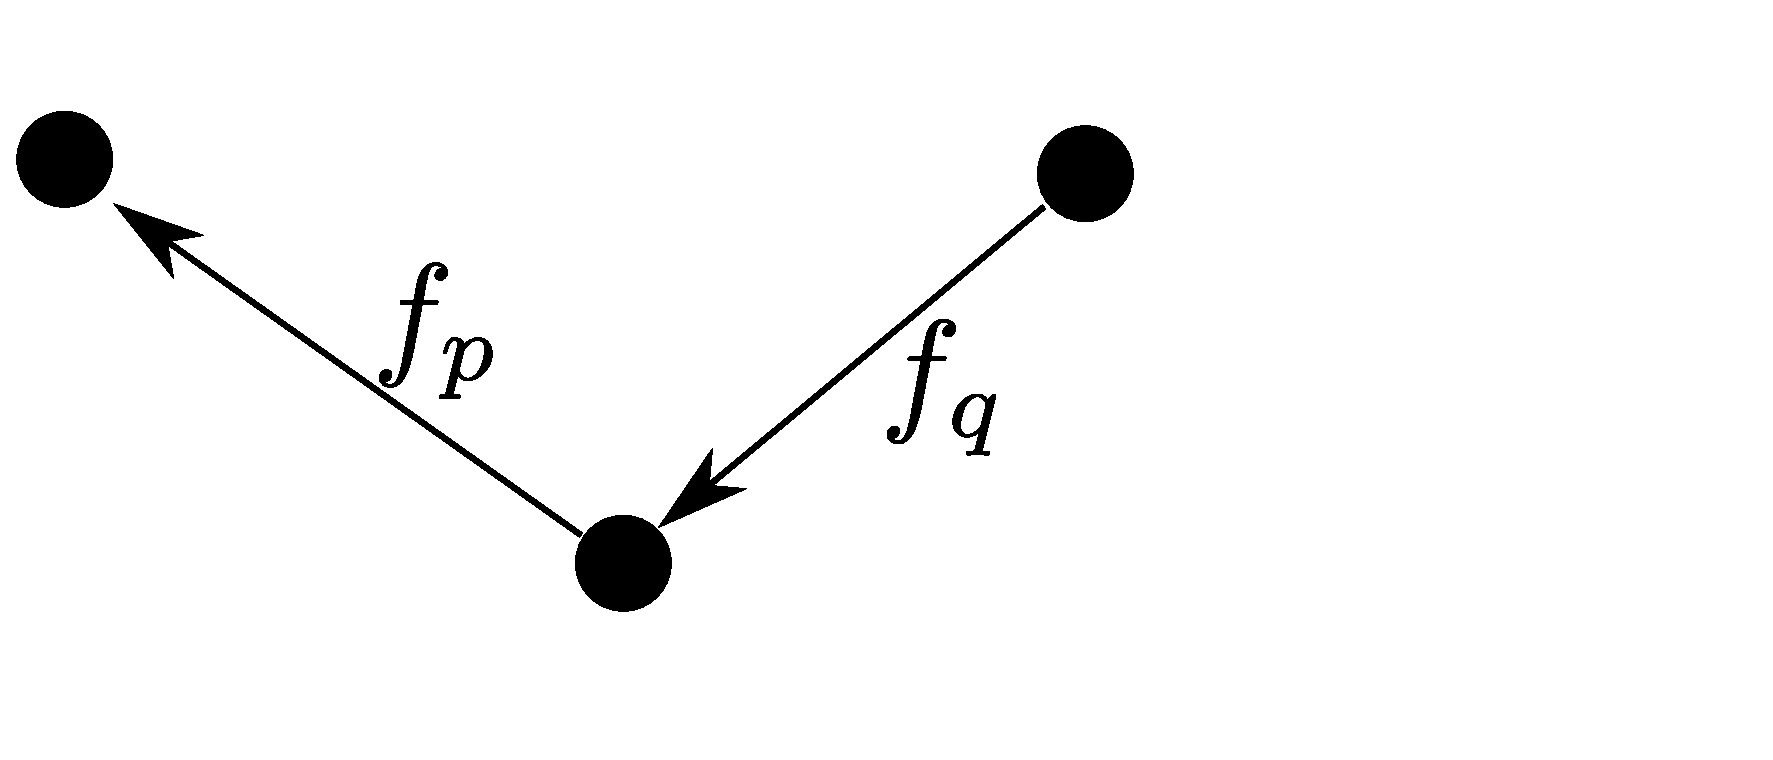
\includegraphics[scale=0.3]{model1.eps}}
\only<2>{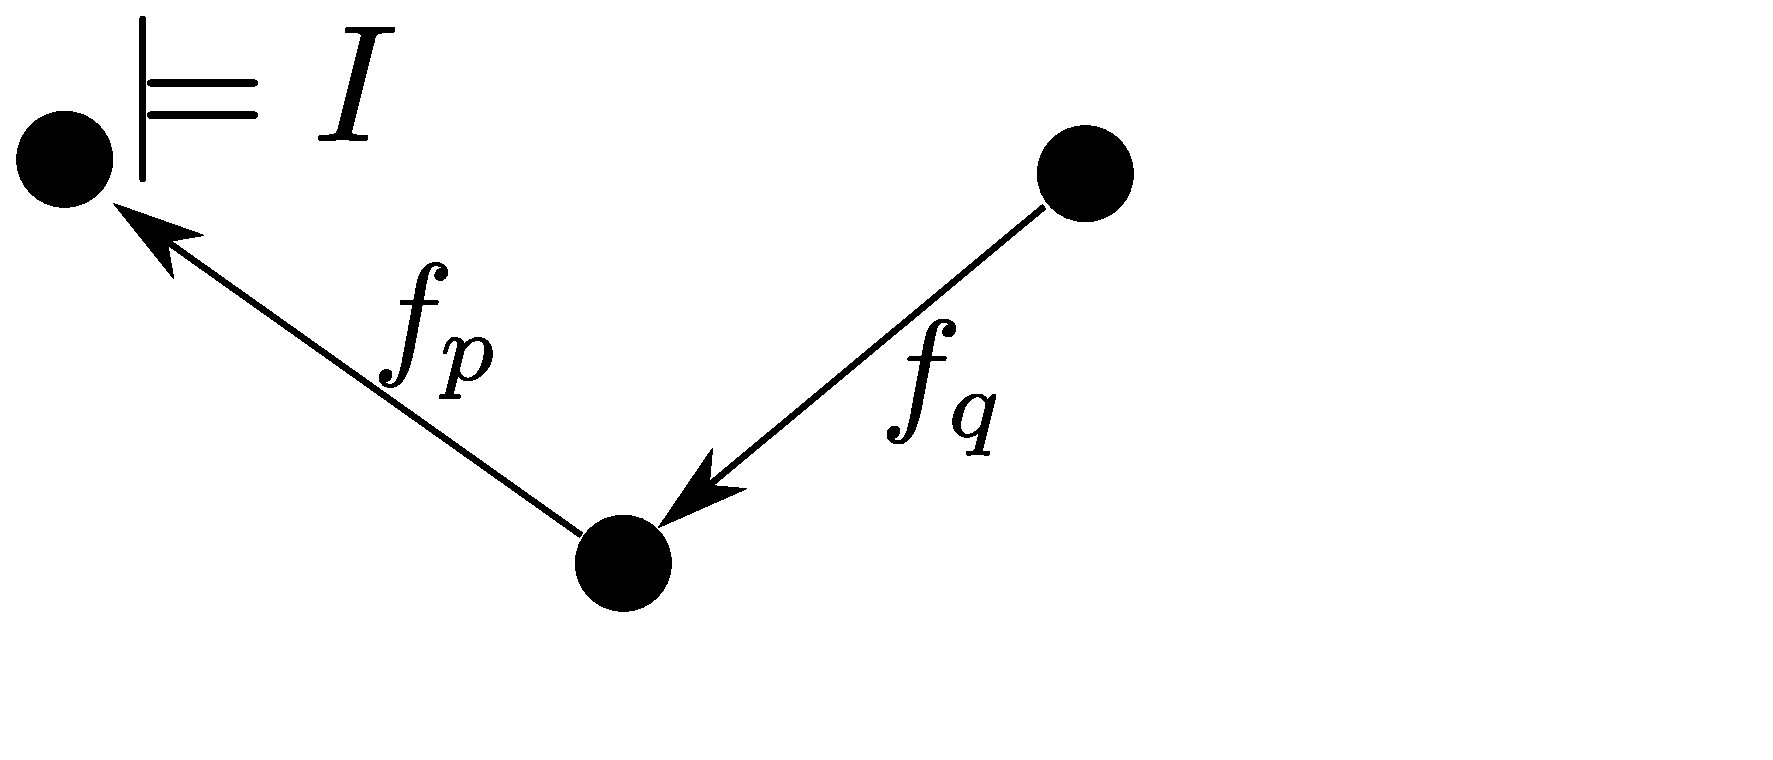
\includegraphics[scale=0.3]{model2.eps}}
\only<3>{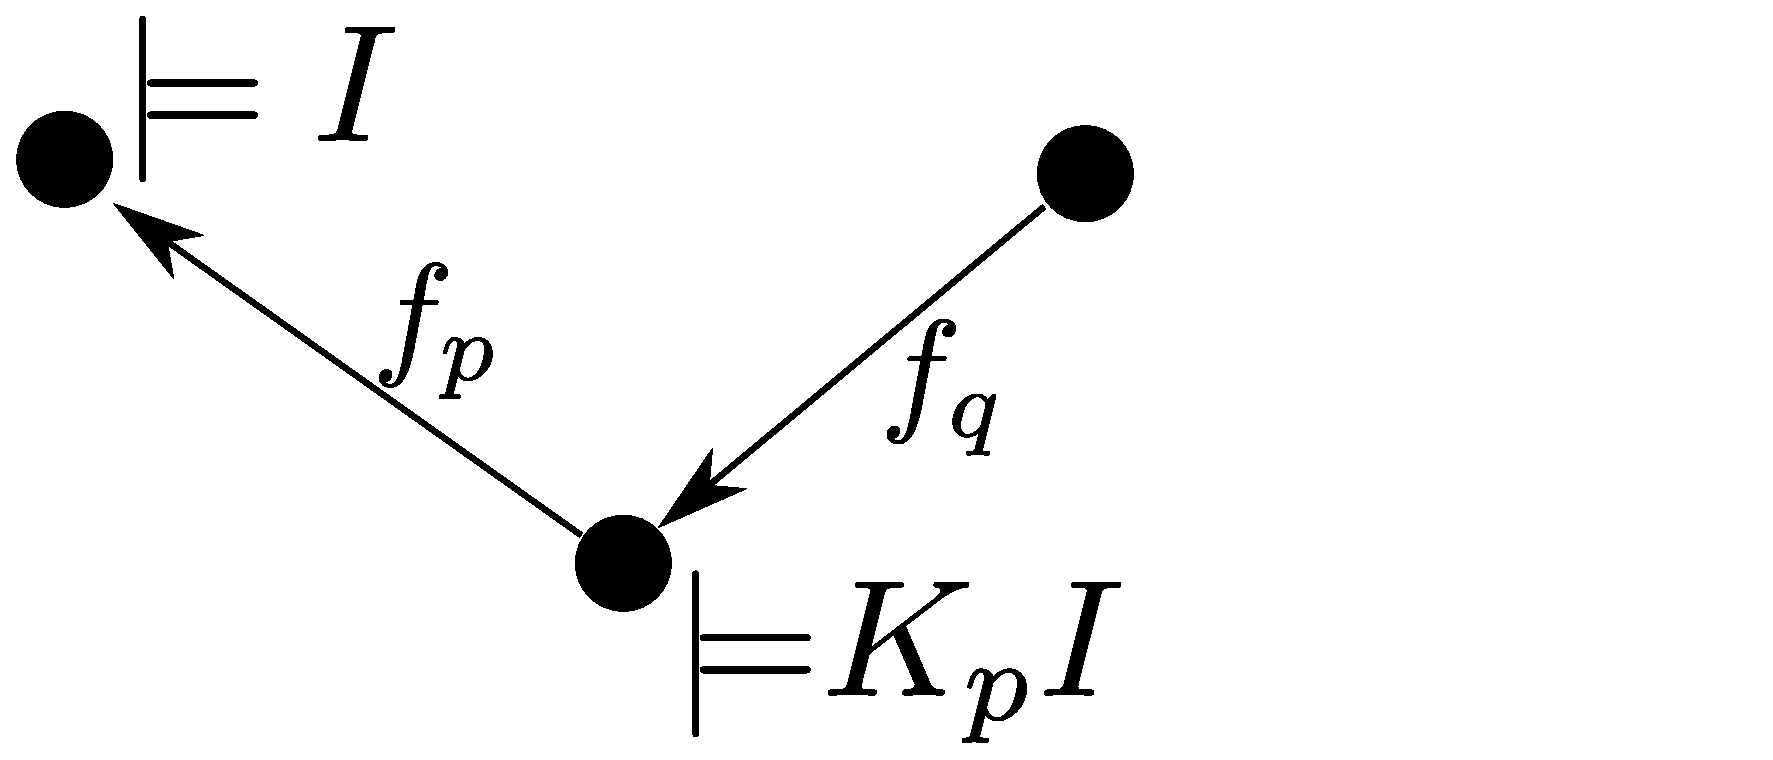
\includegraphics[scale=0.3]{model3.eps}}
\only<4>{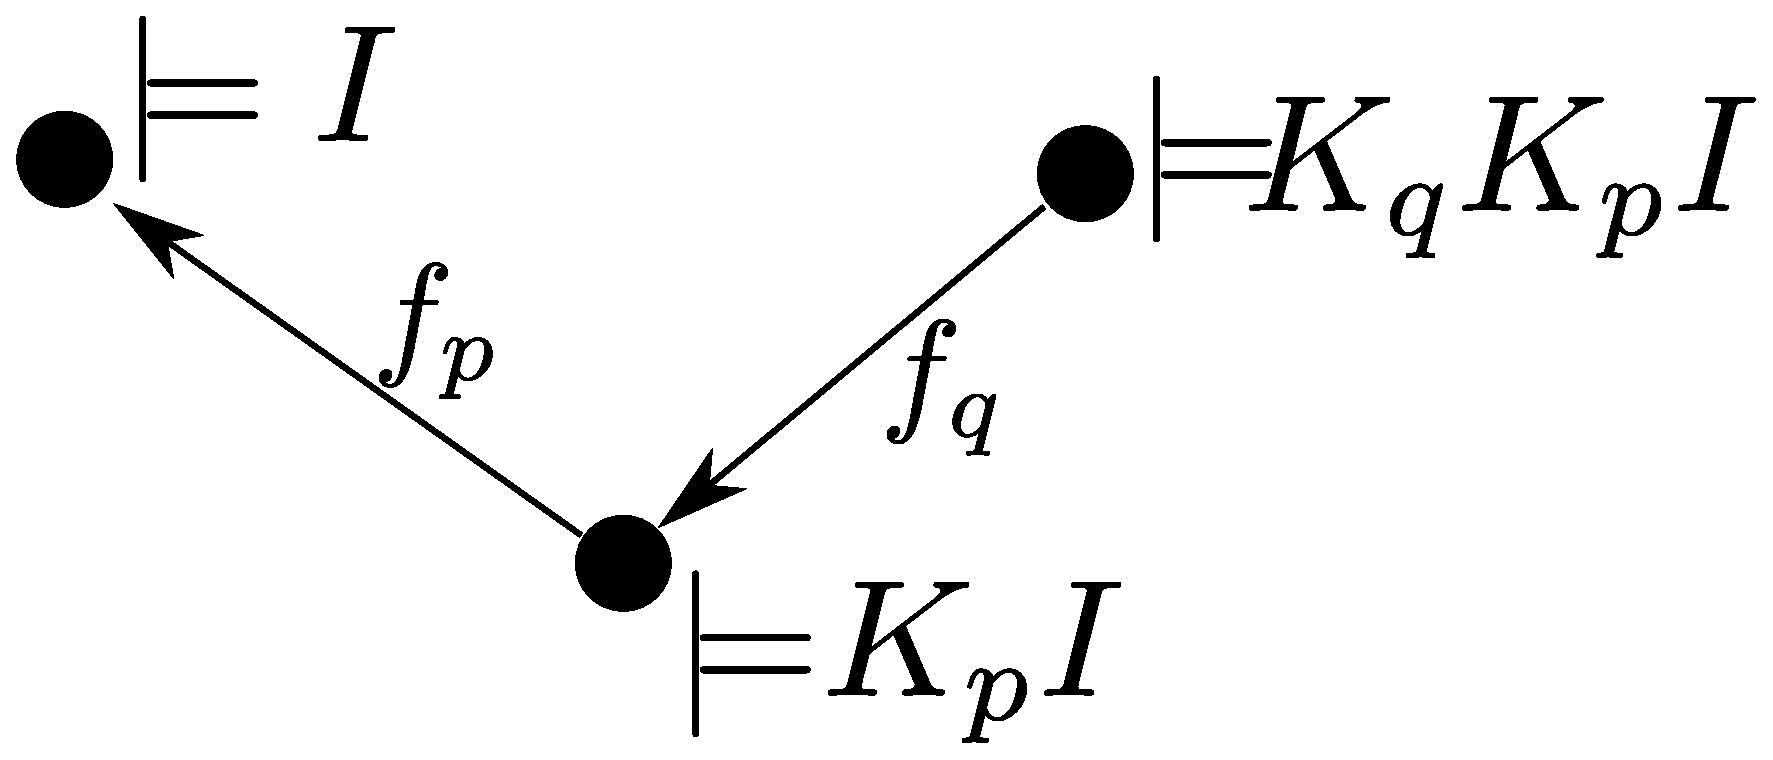
\includegraphics[scale=0.3]{model4.eps}}
\only<5>{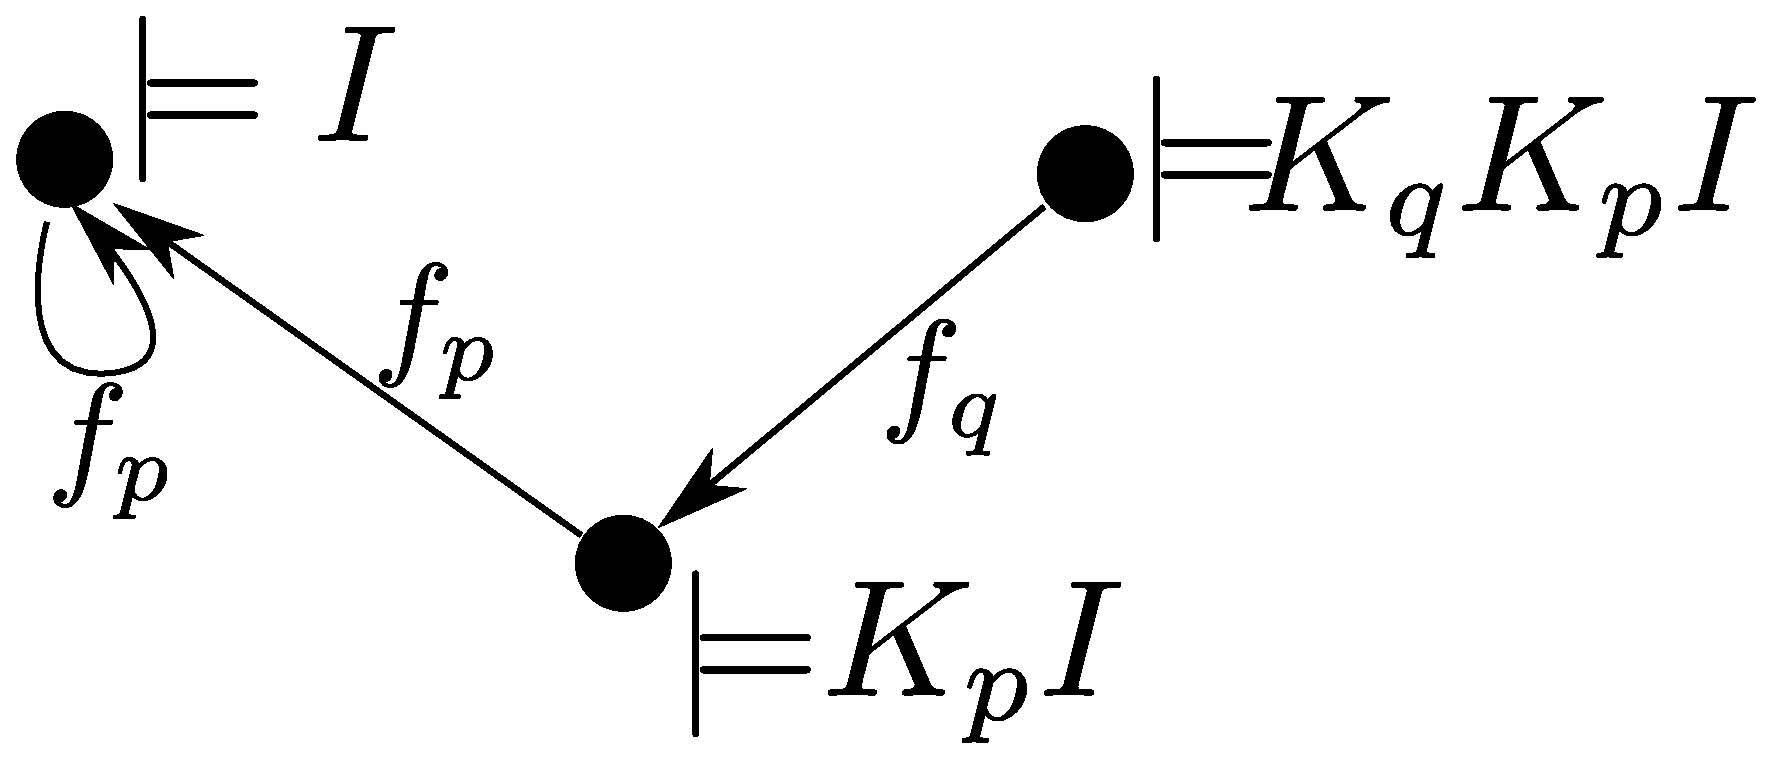
\includegraphics[scale=0.3]{model5.eps}}
\vfill
 \end{frame}

\begin{frame}
 \frametitle{Sequential Consistency of Shared Memory}

For two memory states, either $\preceq$ or $\succeq$ holds.
\vfill

\only<1>{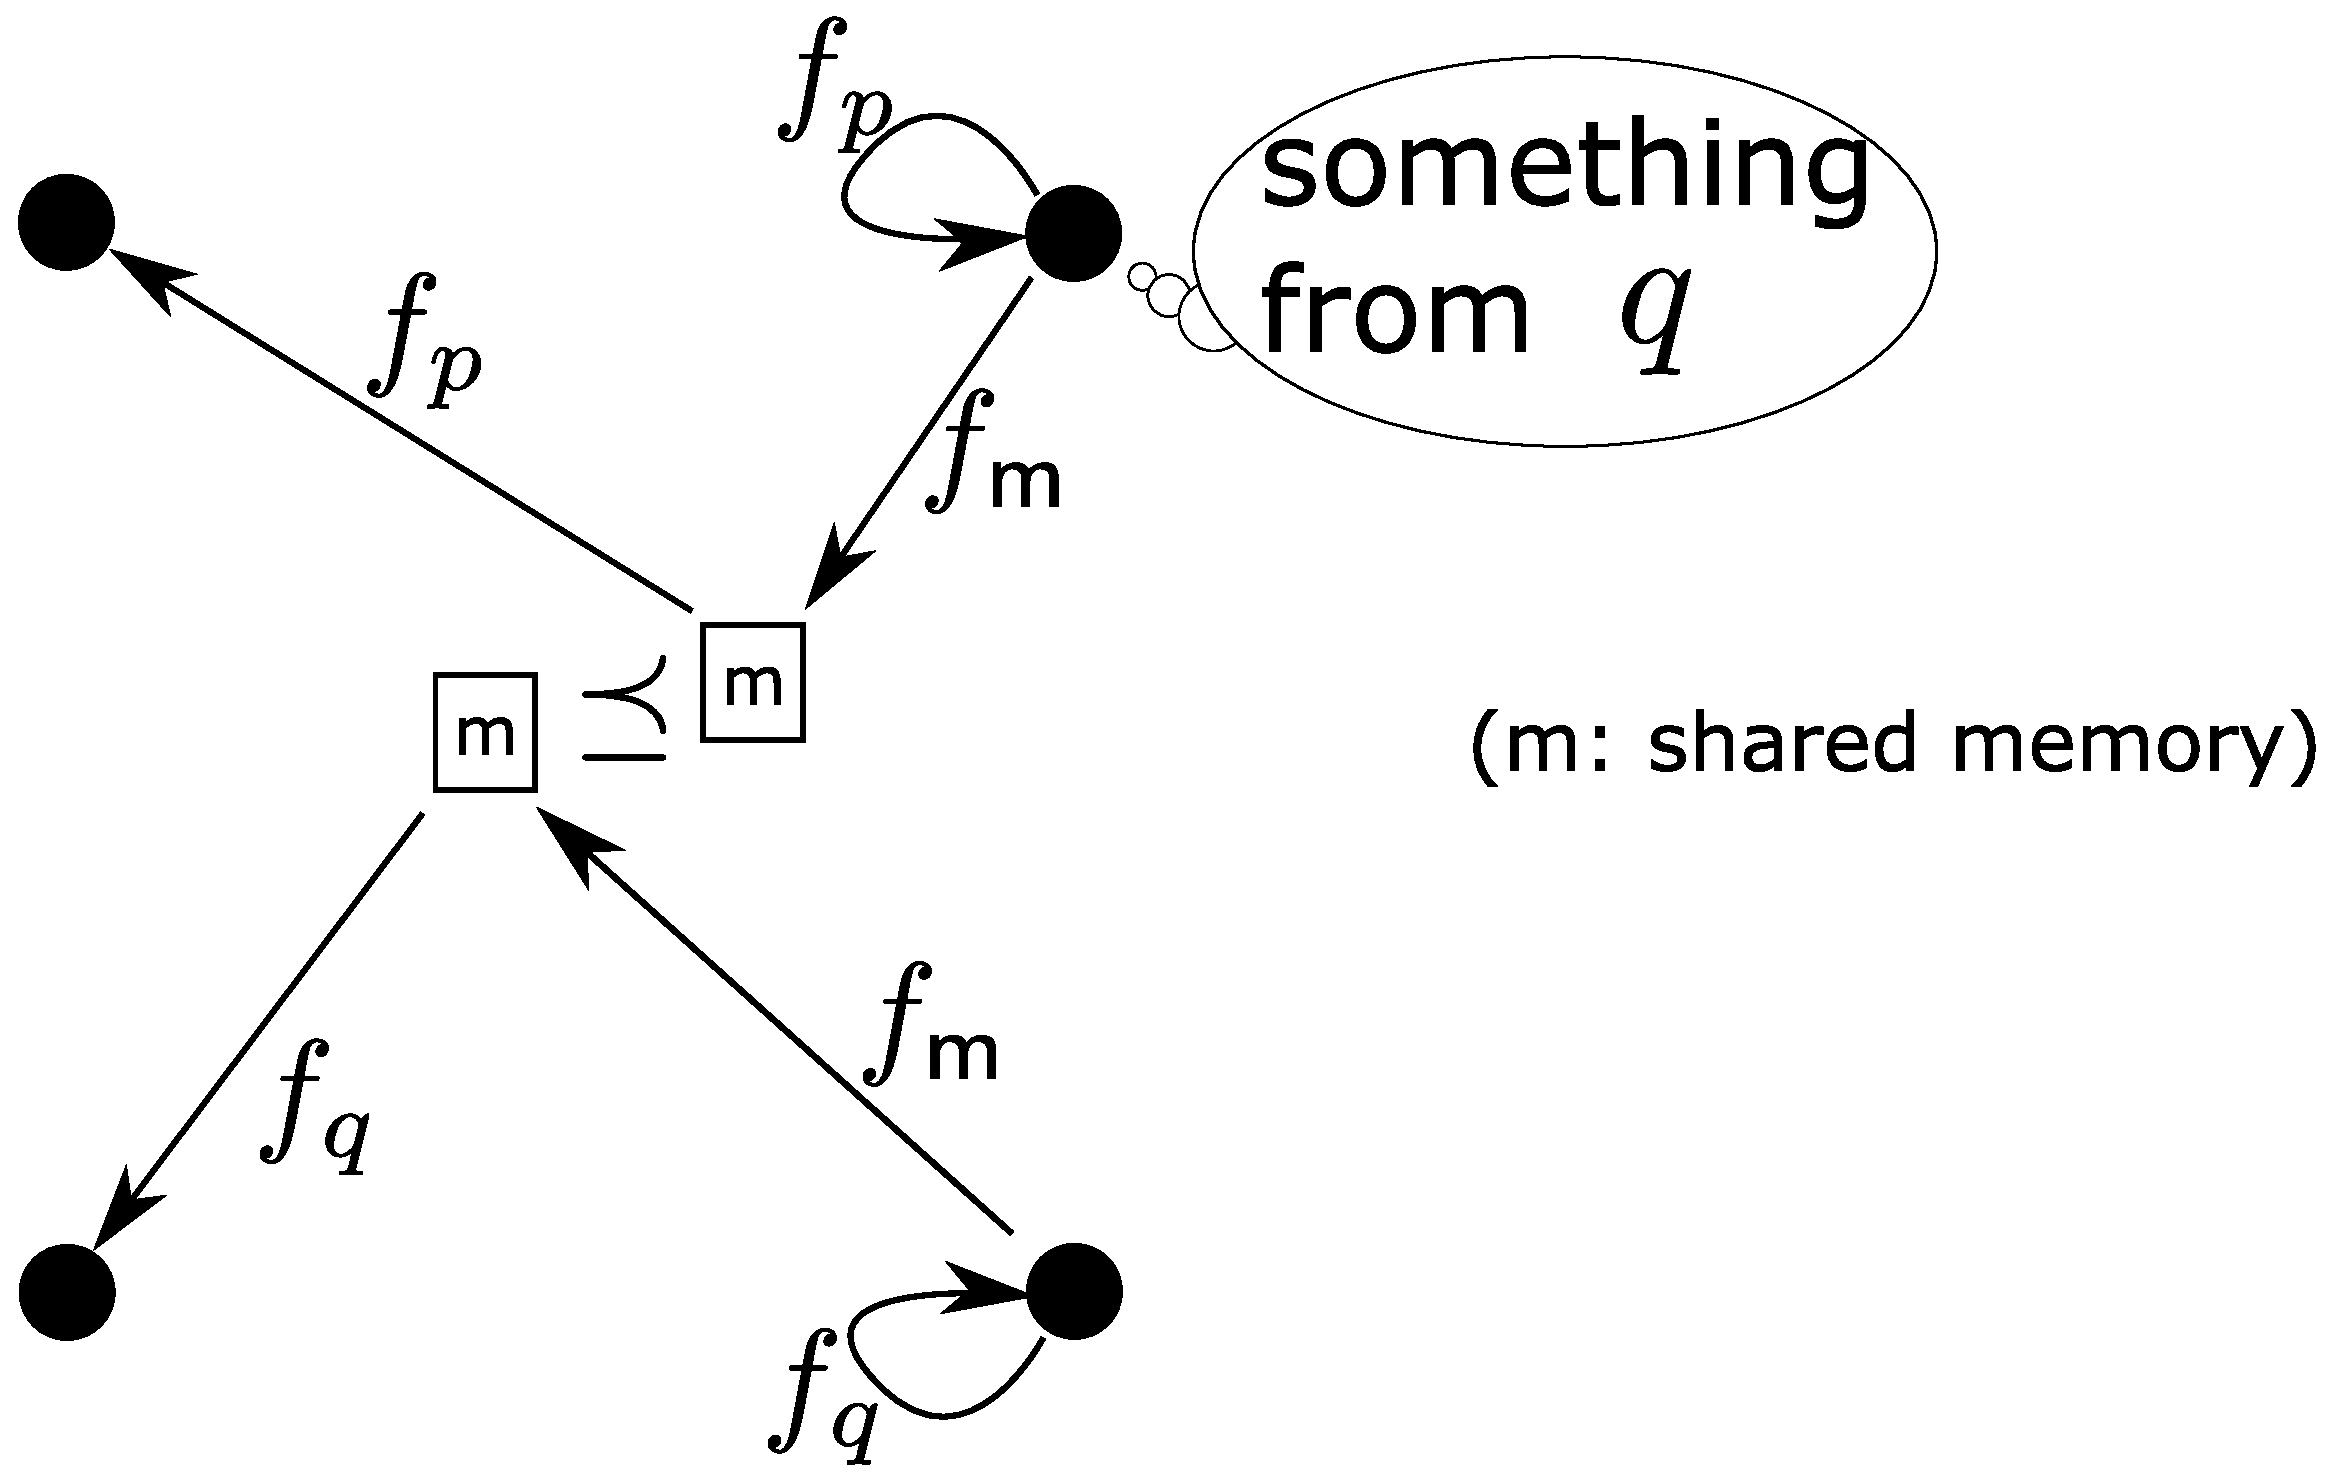
\includegraphics[scale=0.2]{seqcon1.eps}}
\only<2>{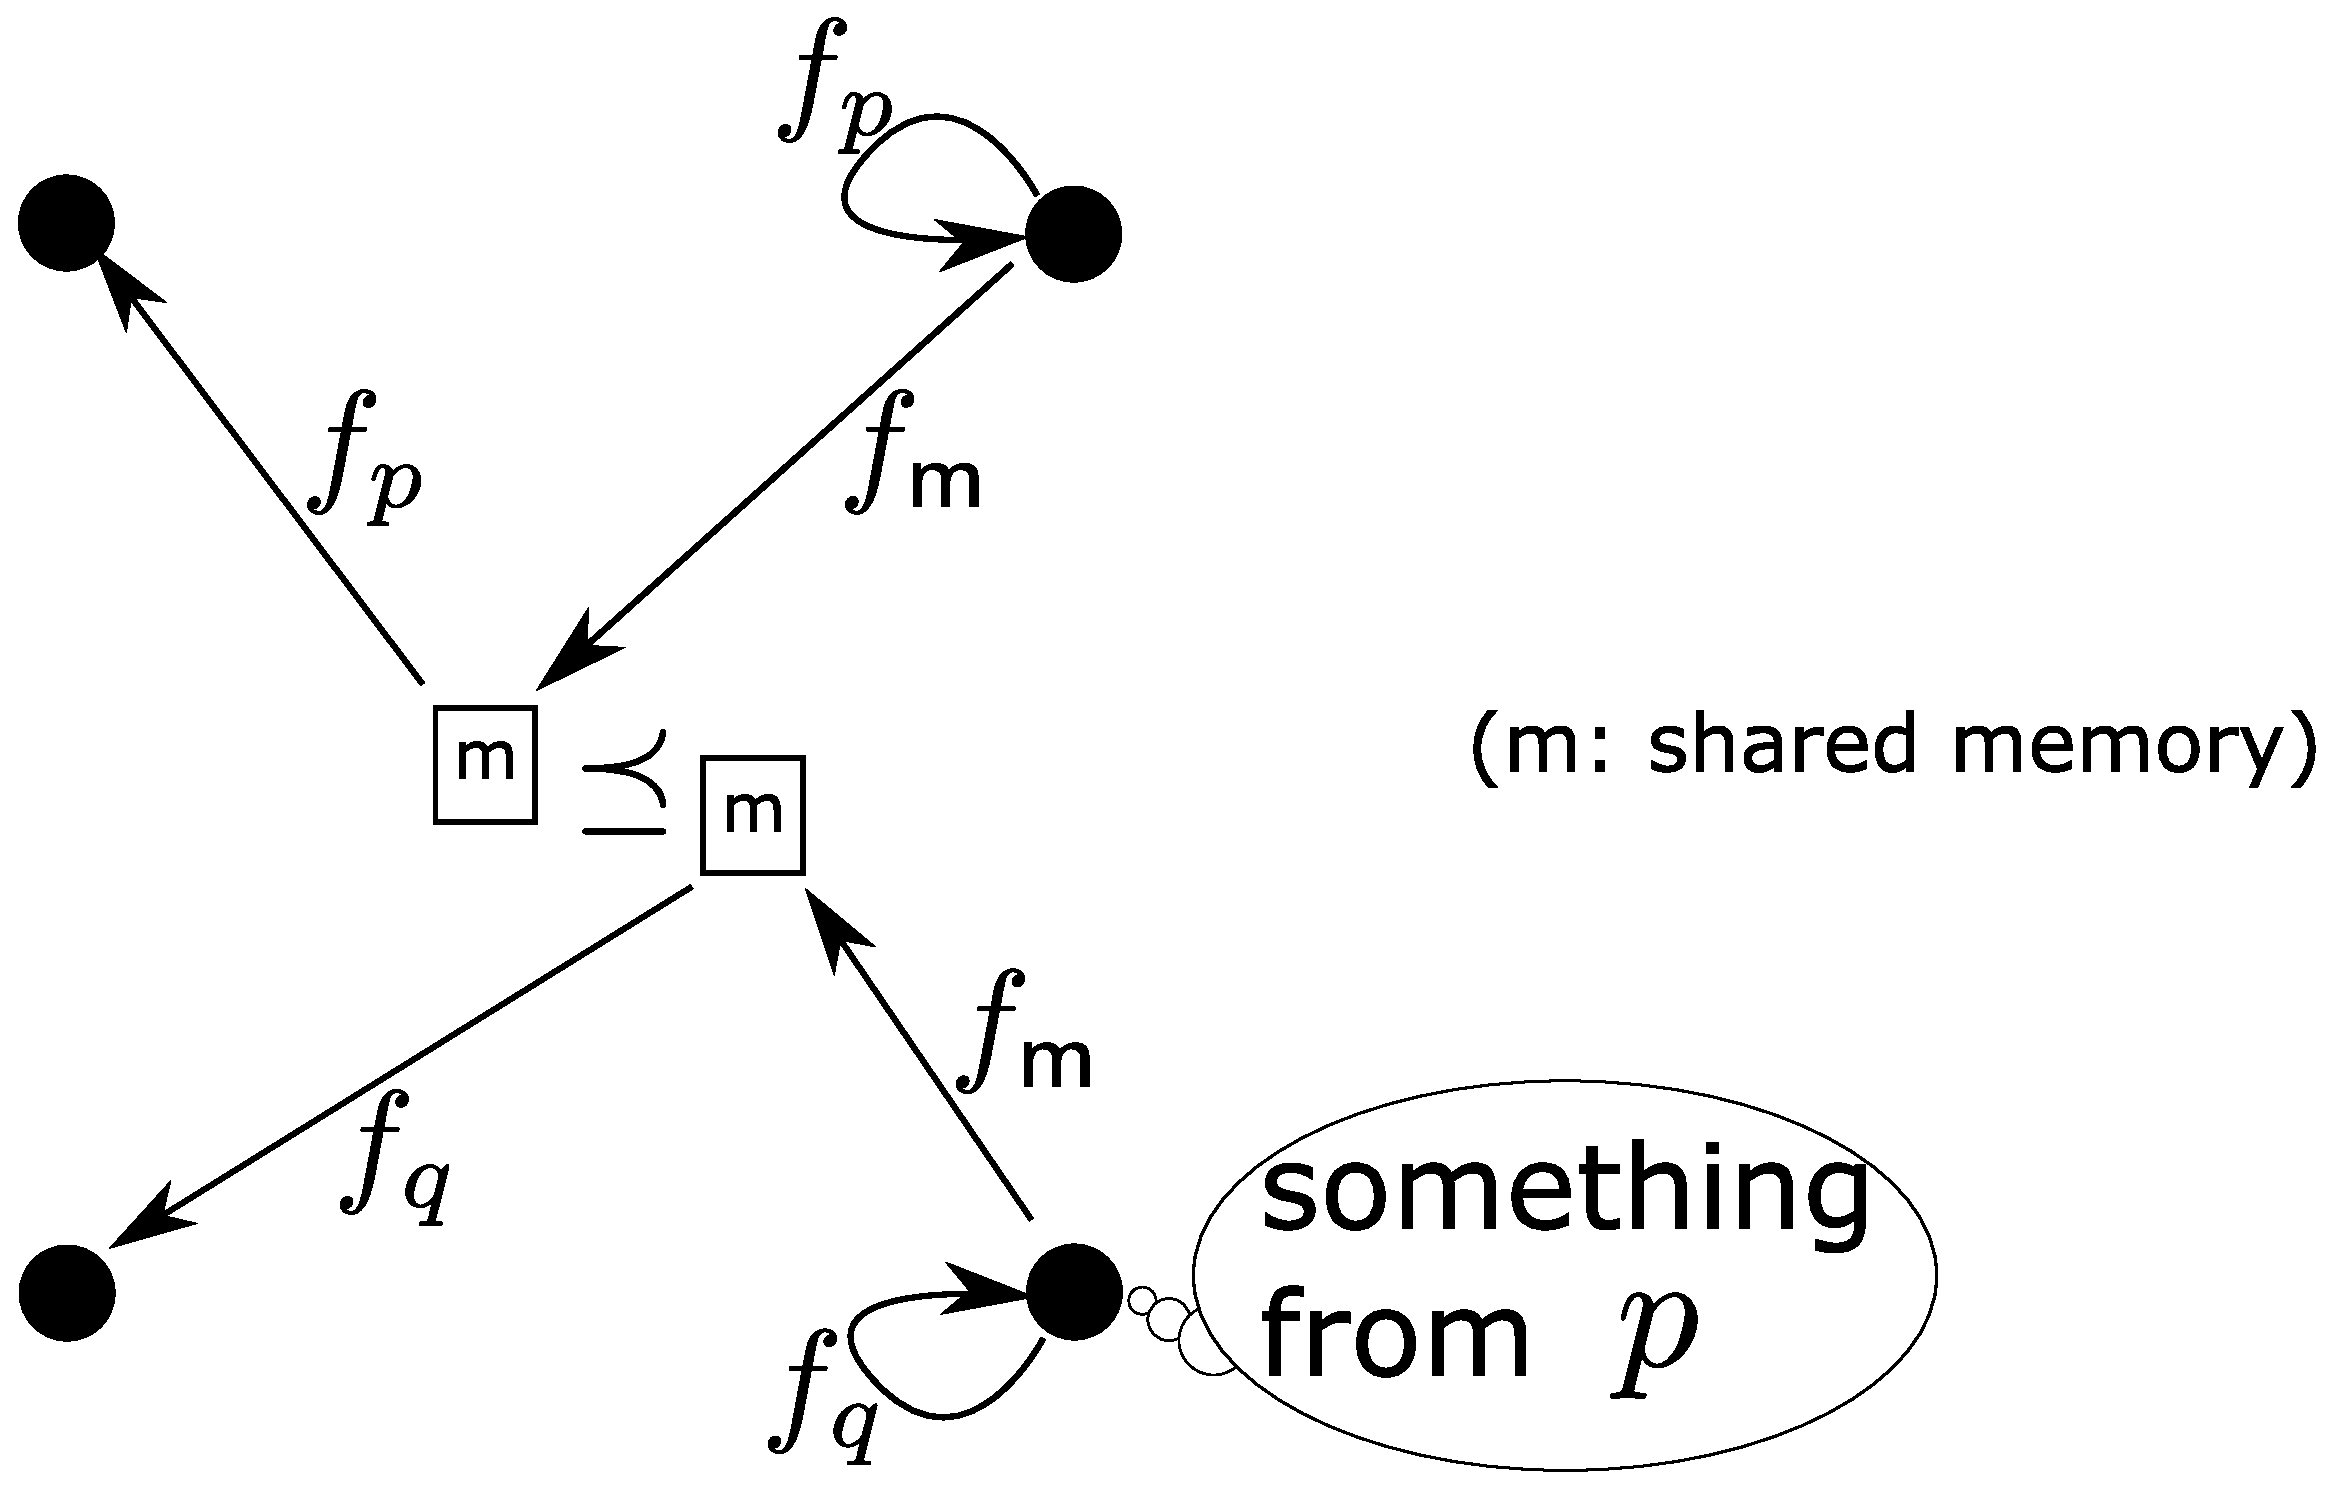
\includegraphics[scale=0.2]{seqcon2.eps}}
\end{frame}

\begin{frame}
 \frametitle{A logic $\mathbf{SC}$ for Sequential Consistency}
   (Hirai, LPAR-16)

 $\mathbf{SC} = \text{Int. {Epistemic} logic}
 + (\alert{K_\memory}\varphi\supset \alert{K_\memory}\psi)\vee
 (\alert{K_\memory}\psi\supset \alert{K_\memory}\varphi)$:\\
 \hskip 2cm Intuitionistic epistemic logic $\subsetneq \mathbf{SC} \subsetneq $ Classical logic

 \vfill
A result:\\
\hskip 2cm $\mathbf{SC}
 \vdash \theta \Longleftrightarrow M\models \theta \text{ for all sequential model }M$
 \vfill
 (Sequential model: for any two \alert{memory states}, $\preceq$ or $\succeq$ holds.)
\end{frame}

 \begin{frame}
\frametitle{An example theorem under sequential consistency} 

 $\vdashsc ((K_p K_m K_p I) \wedge K_q K_m K_q J) \supset 
 ((K_q K_p I) \vee K_p K_q J)$

\vskip 7mm

\structure{Informal reading}
\begin{itemize}
 \item $p$ sends a proof of $I$ to $m$, then $m$ replies to $p$.
 \item $q$ sends a proof of $J$ to $m$, then $m$ replies to $q$.
 \item then, $p$'s knowledge has been transmitted to $q$,\\
       or $q$'s knowledge has been transmitted to $p$.
\end{itemize}
\end{frame}

  \begin{frame}
   \vfill
   If you are interested in propositinoal logics and computation,\\
   try lambda calculi!  (or logic programming?)
   \vfill
  \end{frame}

  \section{Lambda Calculi}

  \begin{frame}
   \frametitle{I did not find $\lambda$, but cut elimination for
   hypersequents}

   Avron's communication rule.

   \fix{add the rule}

   \vfill
   There were works on natural deduction, but no reductions were given.
   They did
   \[
    \text{nd} \rightarrow \text{hyperseq
   with cuts} \rightarrow \text{ hyperseq without cuts} \rightarrow
   \text{normal form nd}
   \]
   \vfill
  \end{frame}

 \begin{frame}
  {
  \frametitle{I had a strong intuition on $(O\rightarrow
  A)\lor (A\rightarrow O)$}
  }

  { Case 1: The car above is faster }
  \only<1>{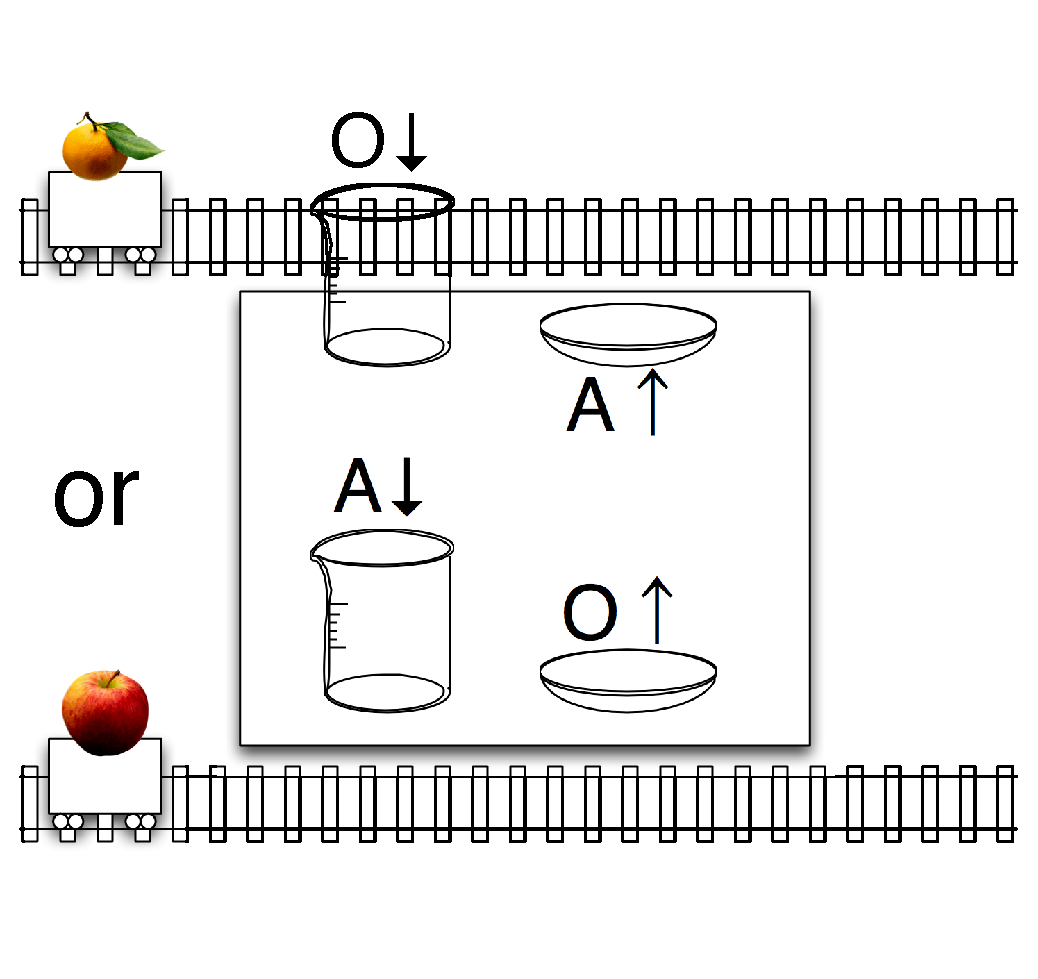
\includegraphics[height=0.8\textheight]{d1.eps}}
  \only<2>{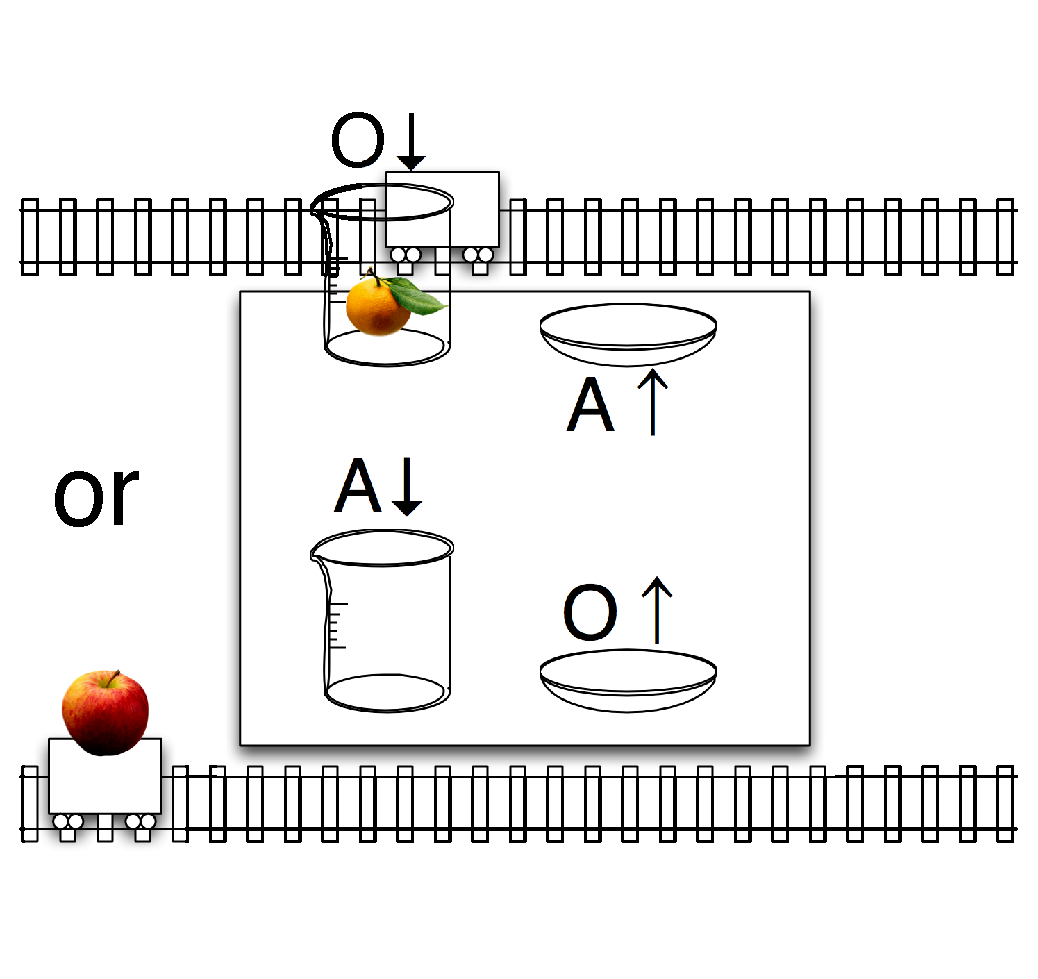
\includegraphics[height=0.8\textheight]{d2.eps}}
  \only<3>{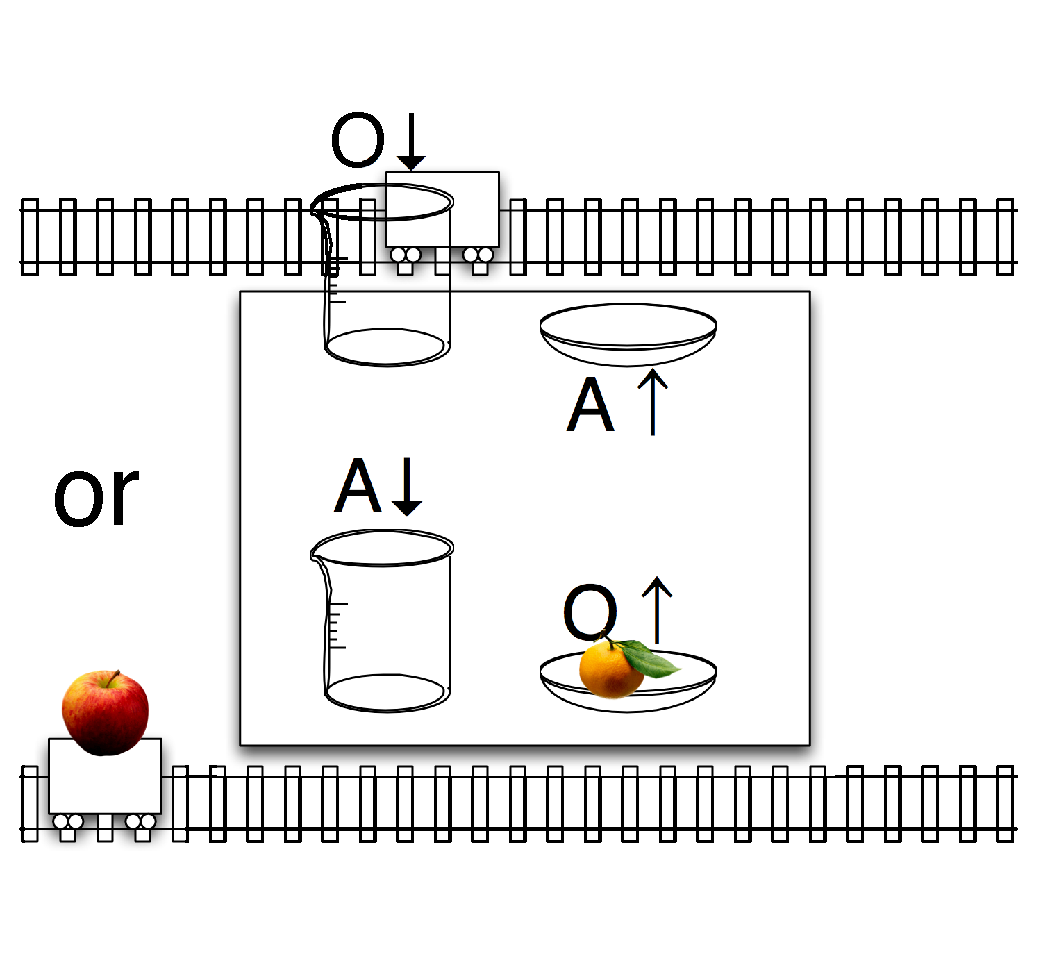
\includegraphics[height=0.8\textheight]{d3.eps}}
  \only<4>{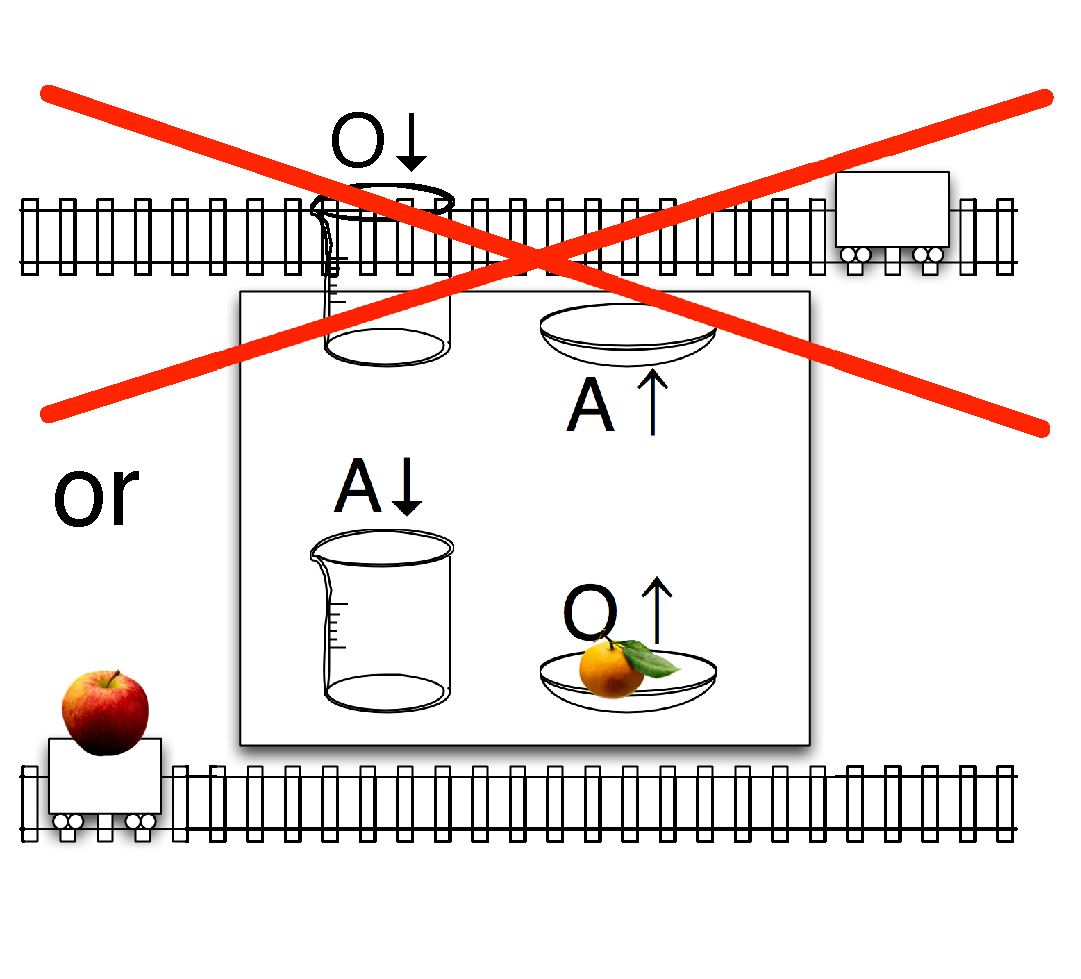
\includegraphics[height=0.8\textheight]{d4.eps}}
  \only<5>{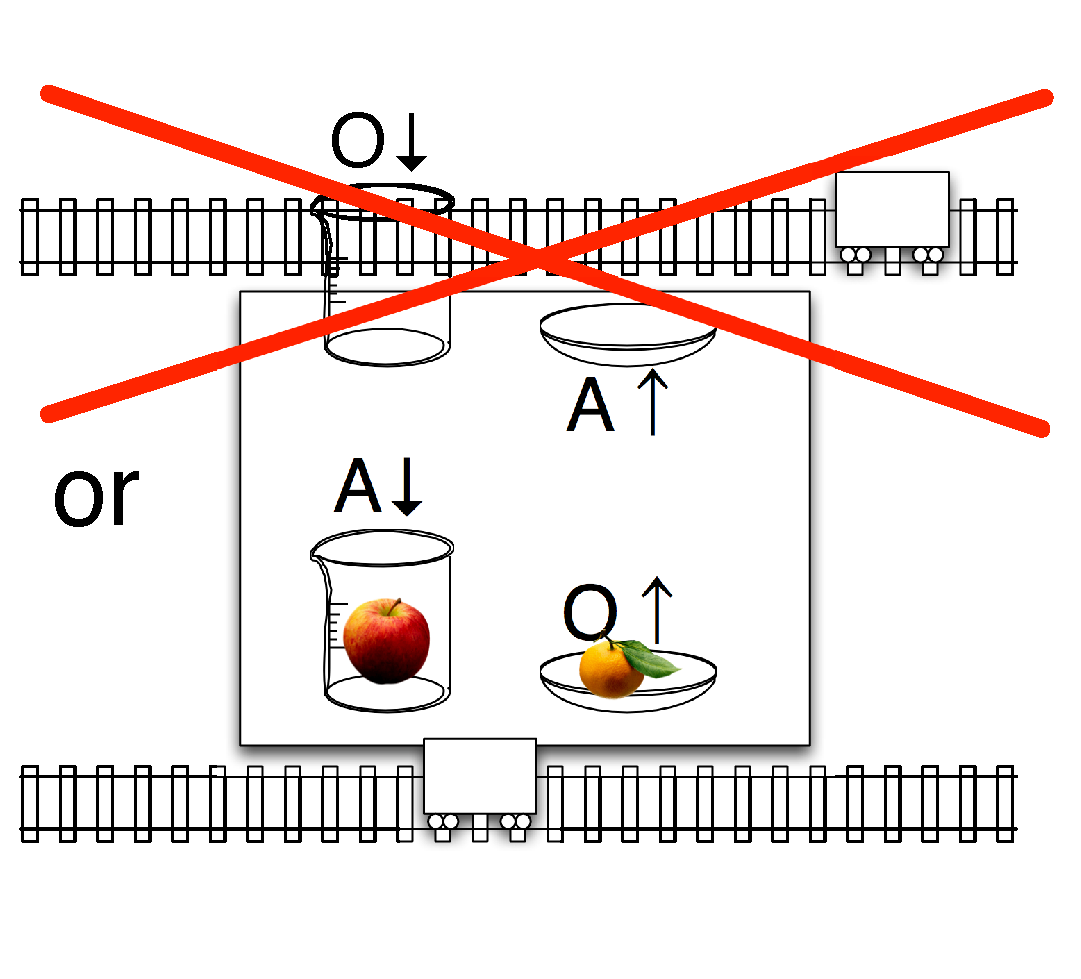
\includegraphics[height=0.8\textheight]{d5.eps}}
  \only<6>{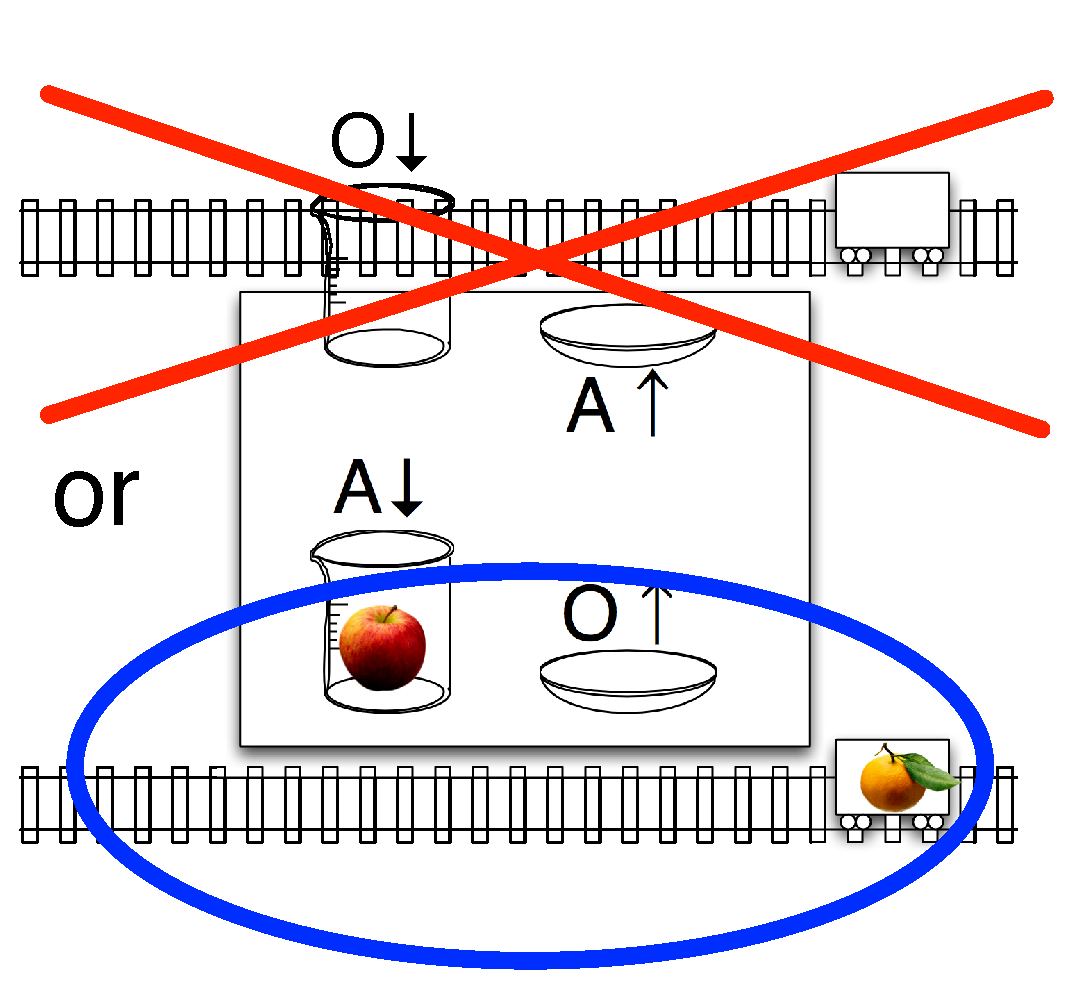
\includegraphics[height=0.8\textheight]{d7.eps}}
 \end{frame}

 \begin{frame}
  {
  \frametitle{I had a strong intuition on $(O\rightarrow
  A)\lor (A\rightarrow O)$}
  }

  { Case 2: The car below is faster}
  \only<1>{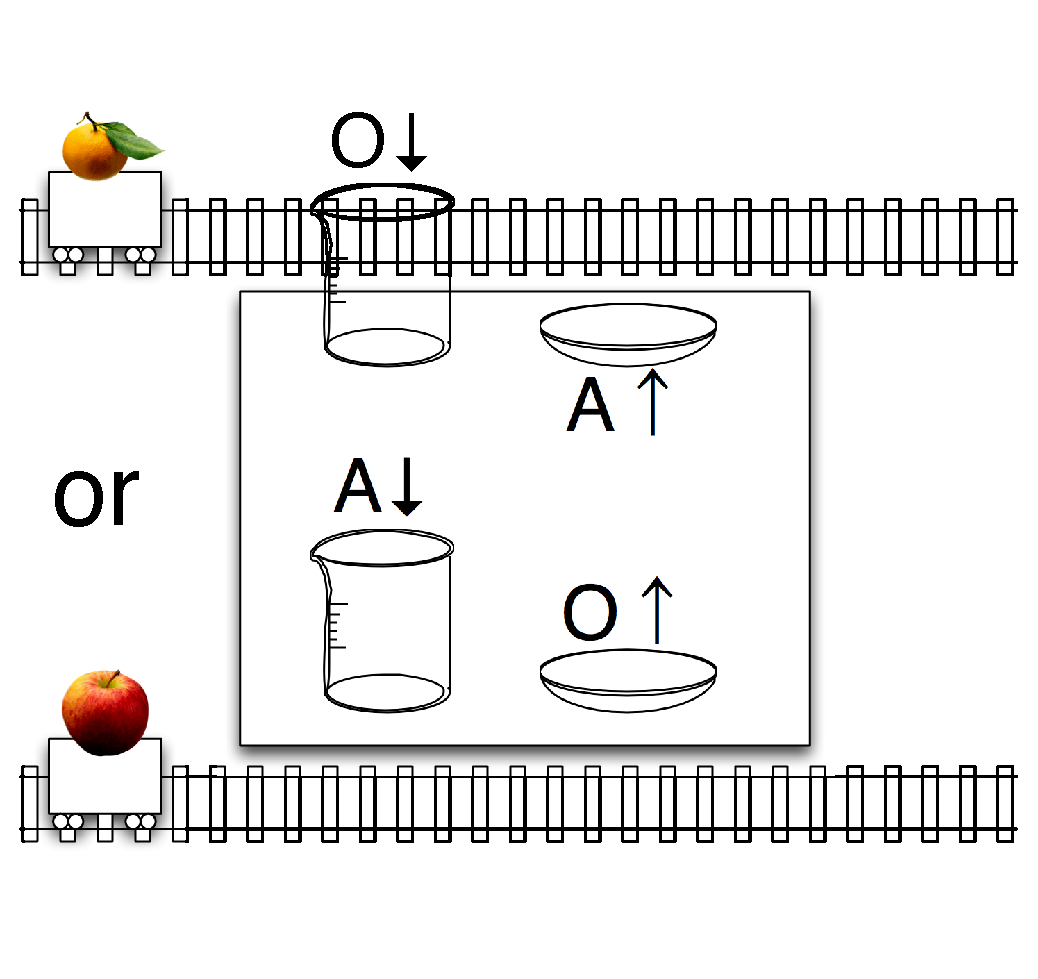
\includegraphics[height=0.8\textheight]{e1.eps}}
  \only<2>{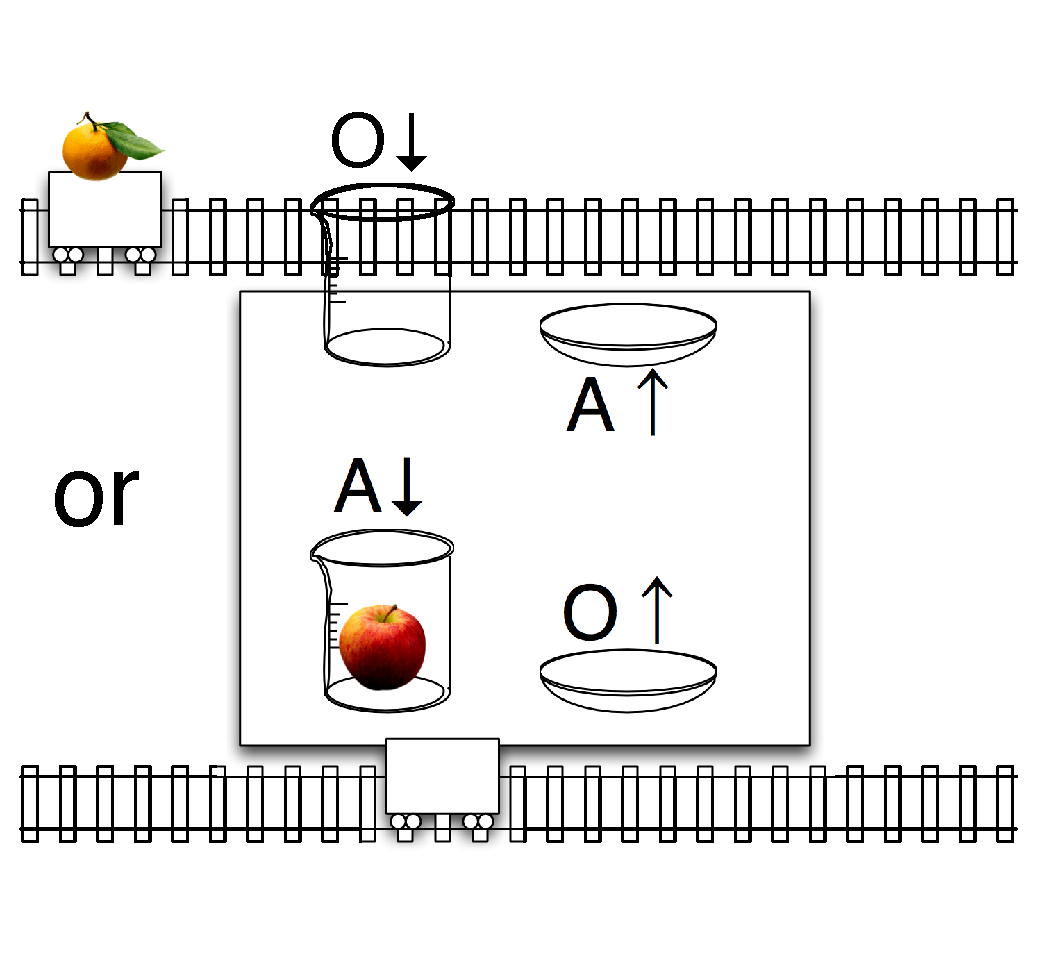
\includegraphics[height=0.8\textheight]{e2.eps}}
  \only<3>{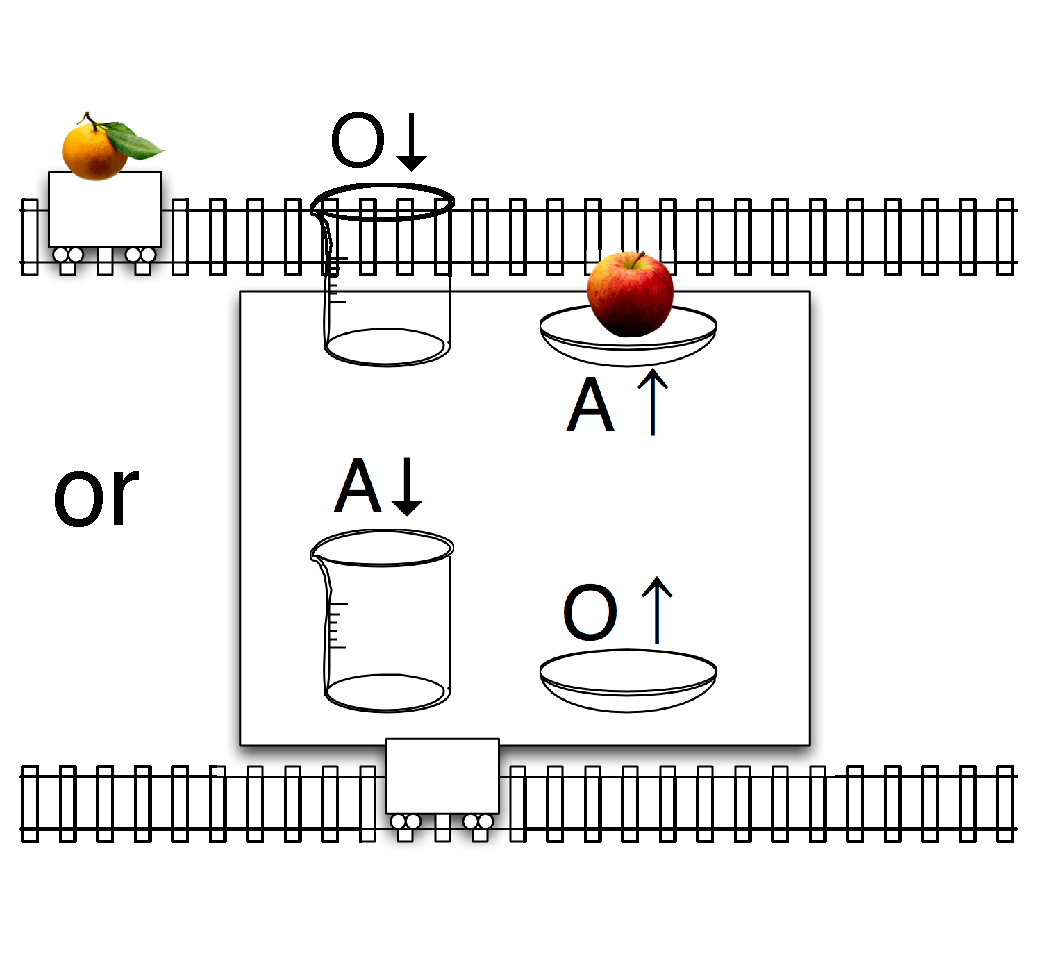
\includegraphics[height=0.8\textheight]{e3.eps}}
  \only<4>{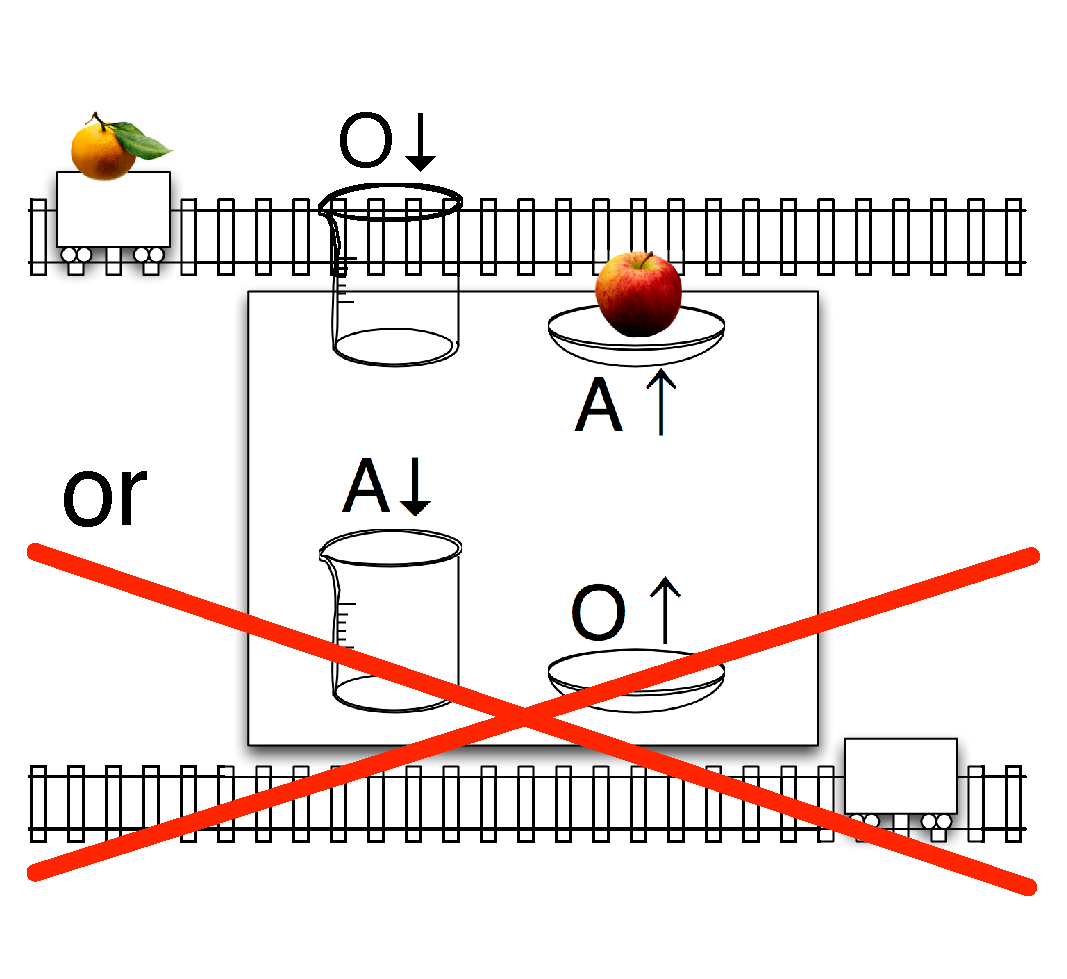
\includegraphics[height=0.8\textheight]{e4.eps}}
  \only<5>{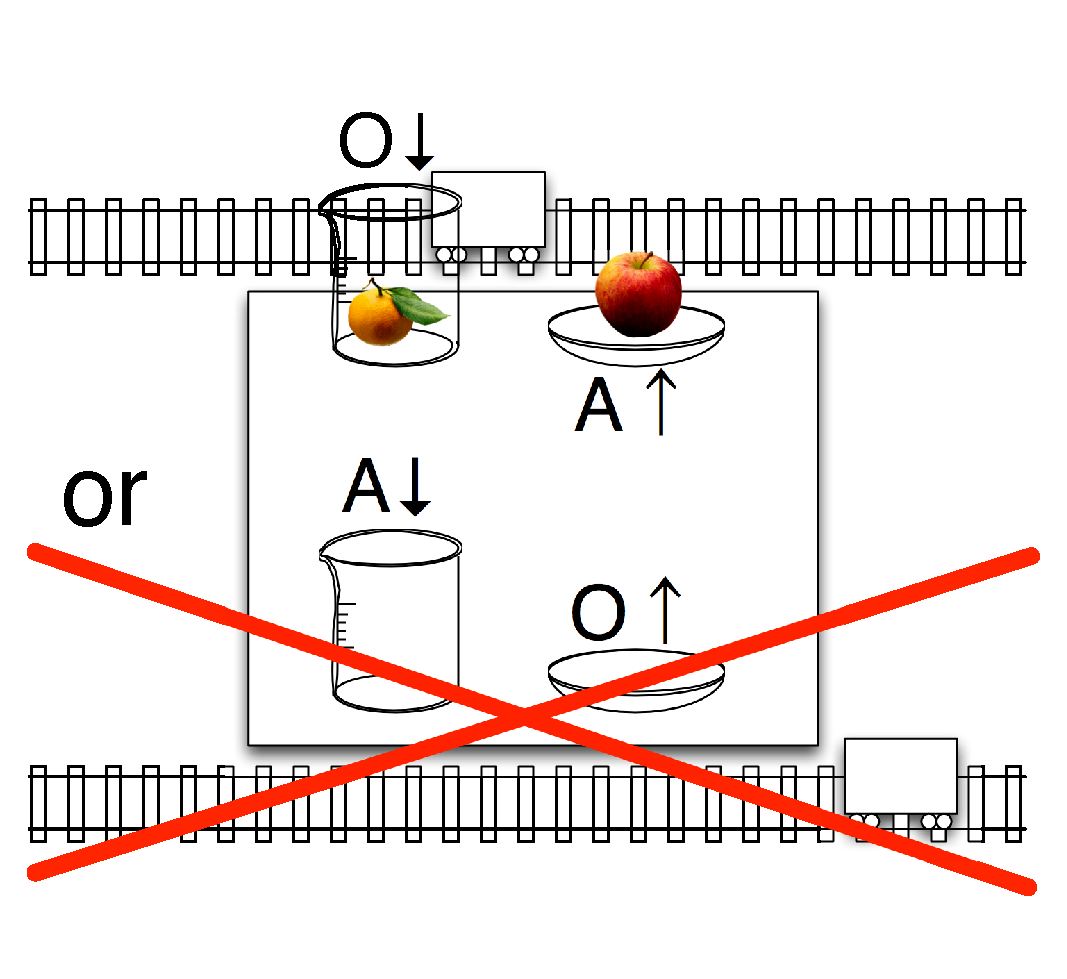
\includegraphics[height=0.8\textheight]{e5.eps}}
  \only<6>{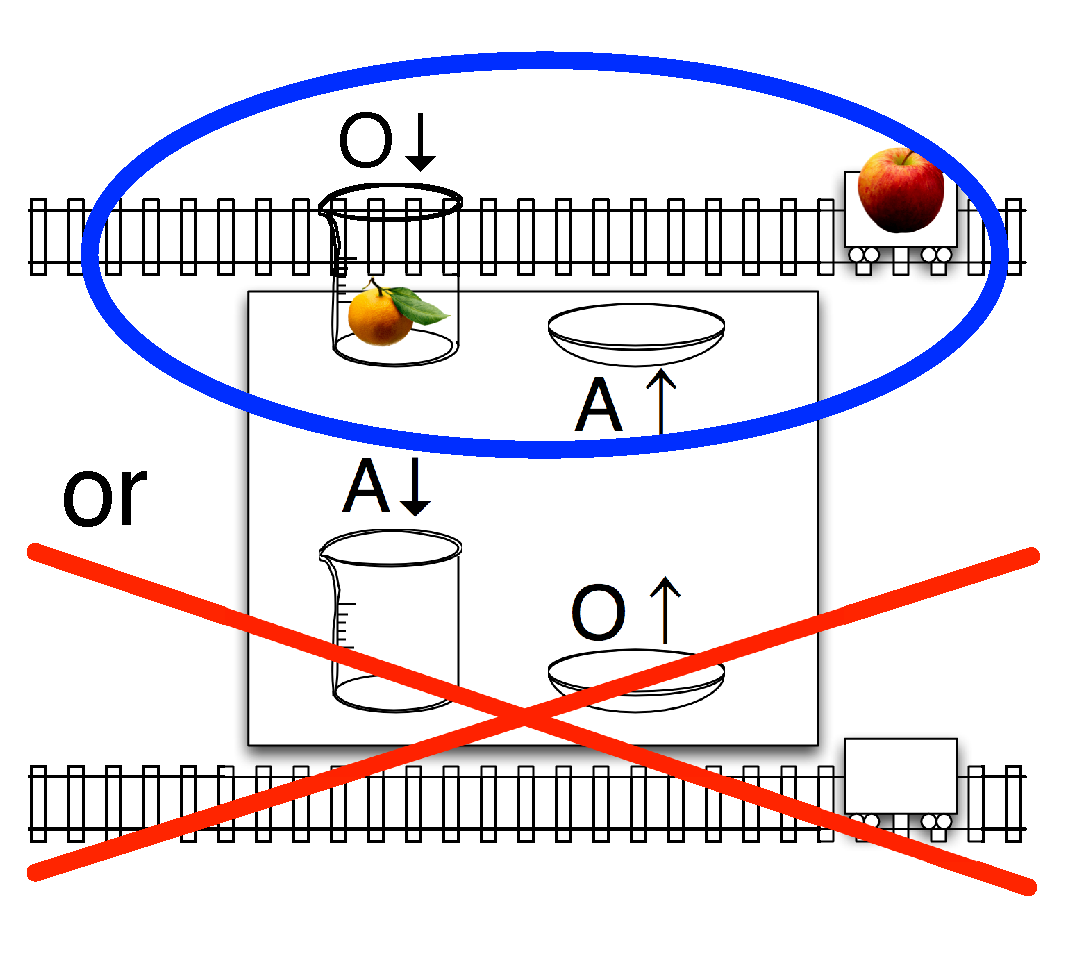
\includegraphics[height=0.8\textheight]{e7.eps}}
 \end{frame}


 \begin{frame}
  \ej{
  \frametitle{I had a strong intuition on $(O\rightarrow
  A)\lor (A\rightarrow O)$}
  }
  {
  \frametitle{ダメット公理$(O\rightarrow  A)\lor (A\rightarrow O)$の計算
  的解釈}
  }

  \ej
  { Case 3: Both cars has about the same speed}
  { 場合3: 両方だいたい揃って動く場合}
  \only<1>{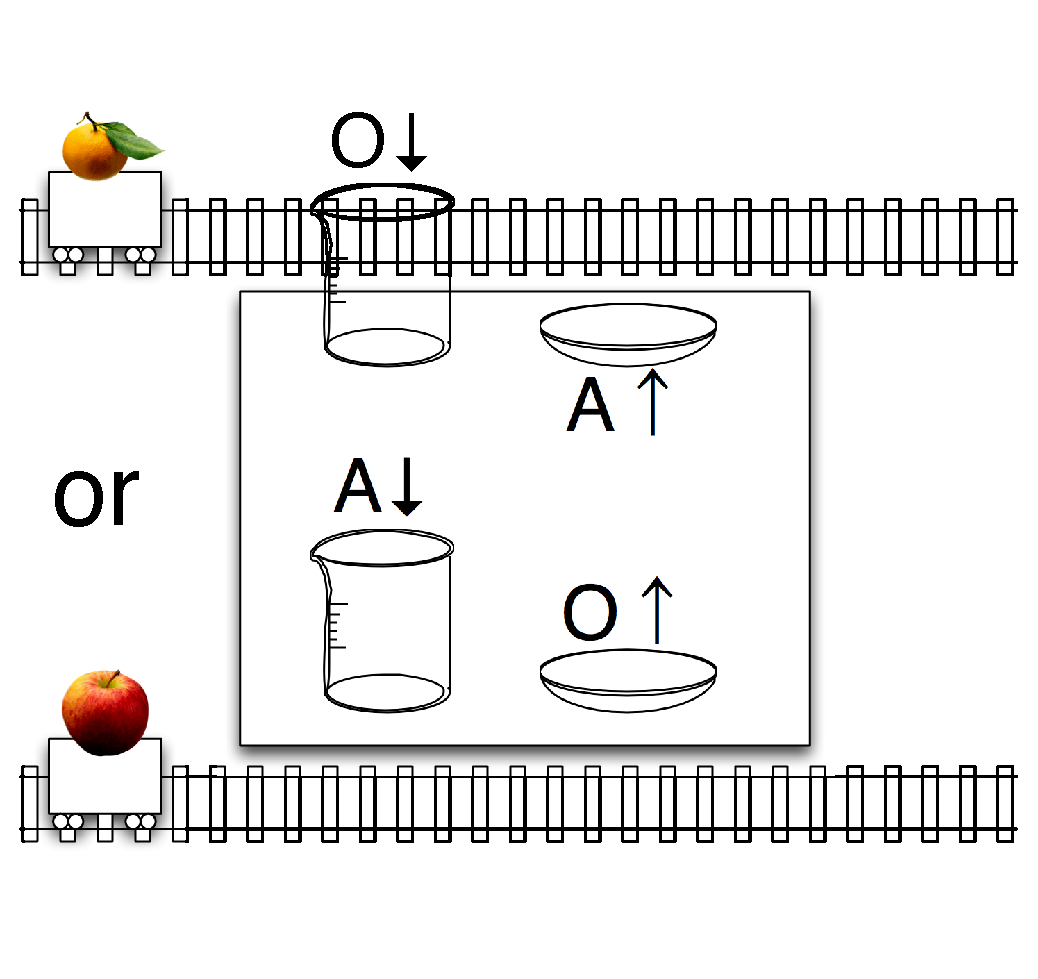
\includegraphics[height=0.8\textheight]{f1.eps}}
  \only<2>{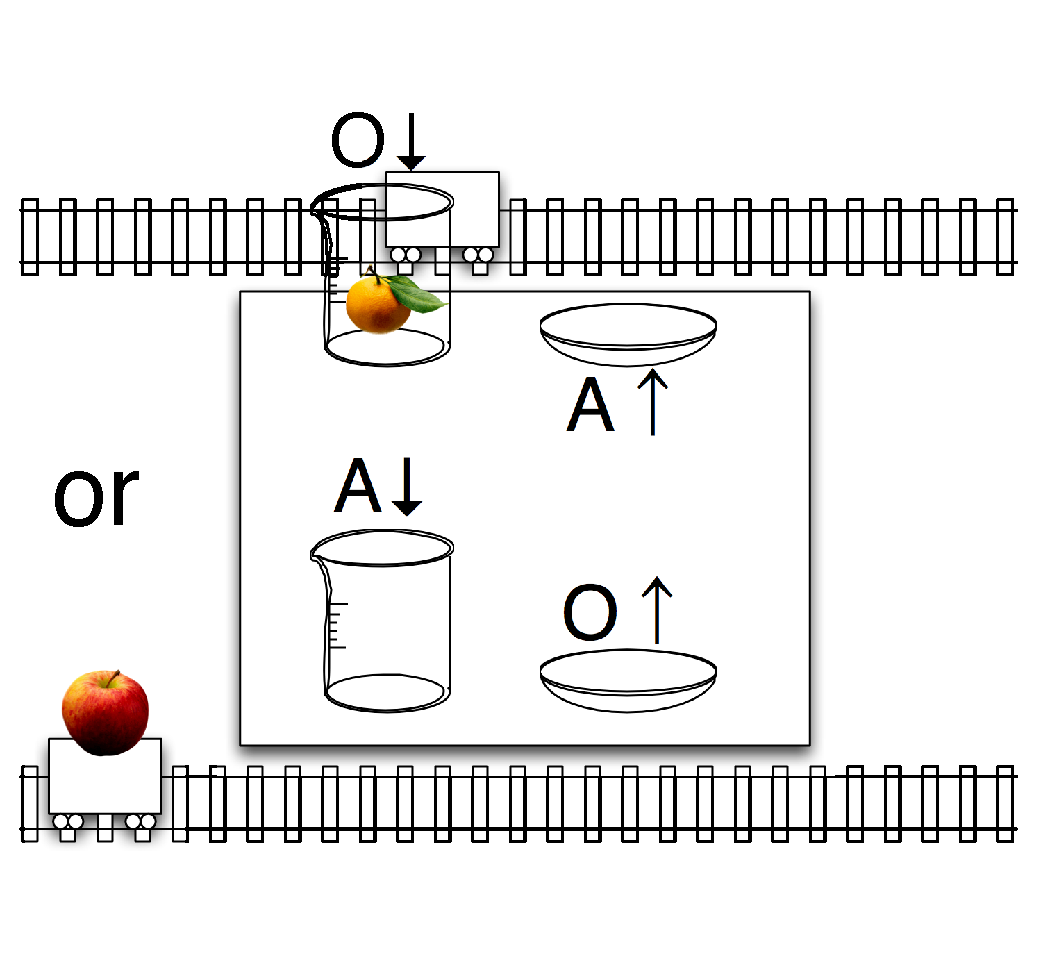
\includegraphics[height=0.8\textheight]{f2.eps}}
  \only<3>{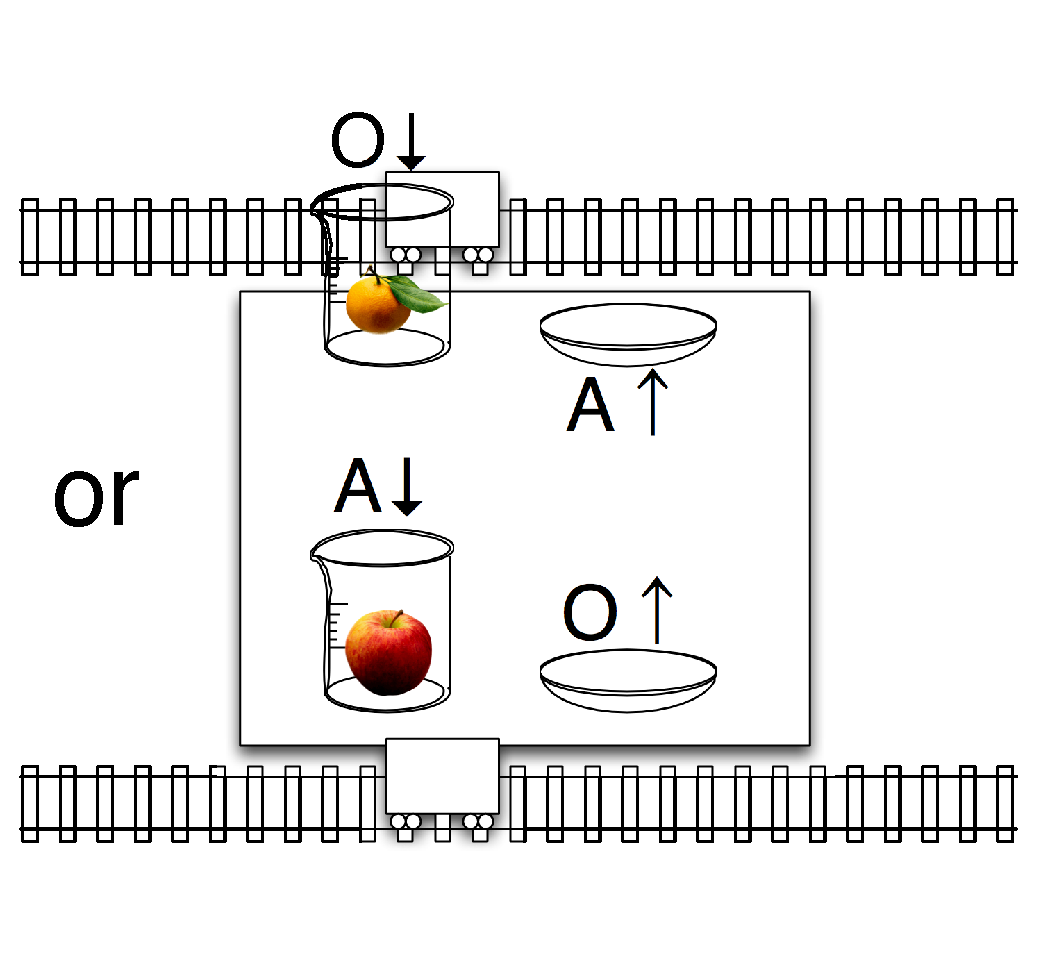
\includegraphics[height=0.8\textheight]{f3.eps}}
  \only<4>{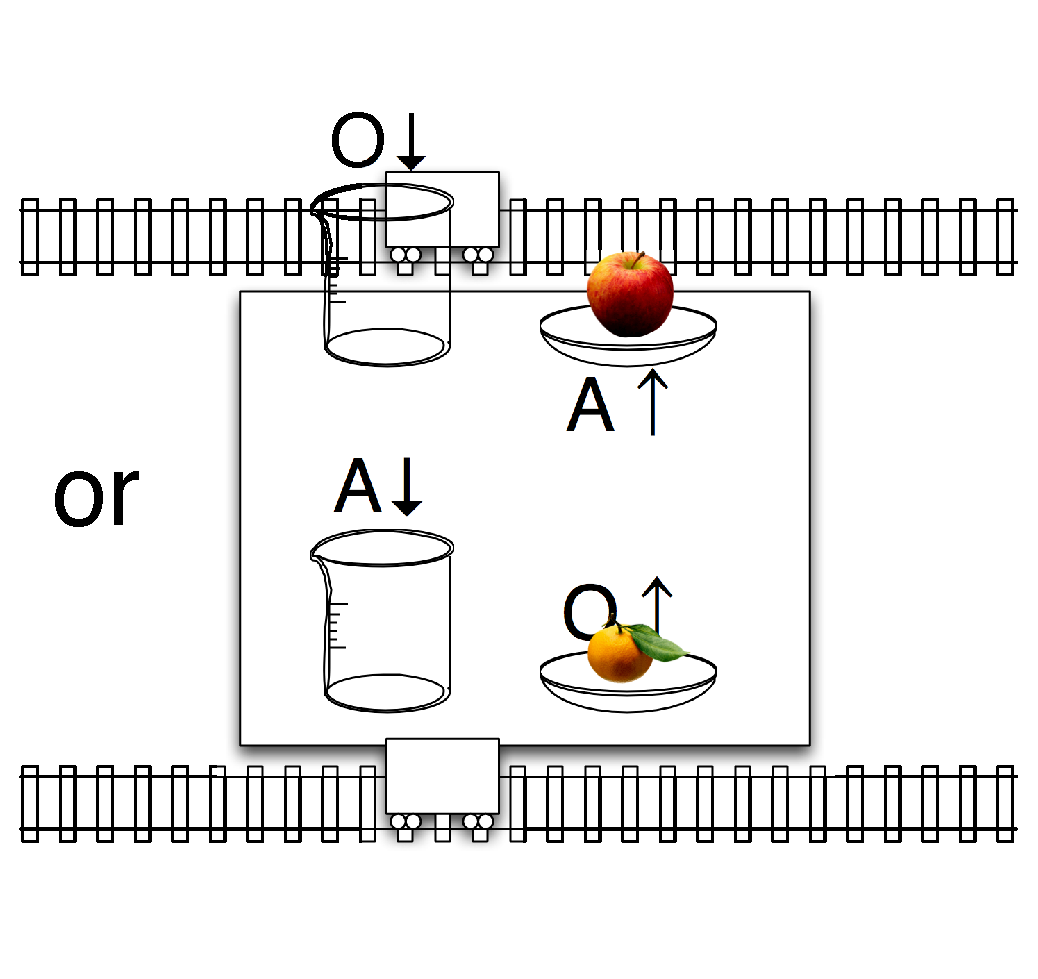
\includegraphics[height=0.8\textheight]{f4.eps}}
  \only<5>{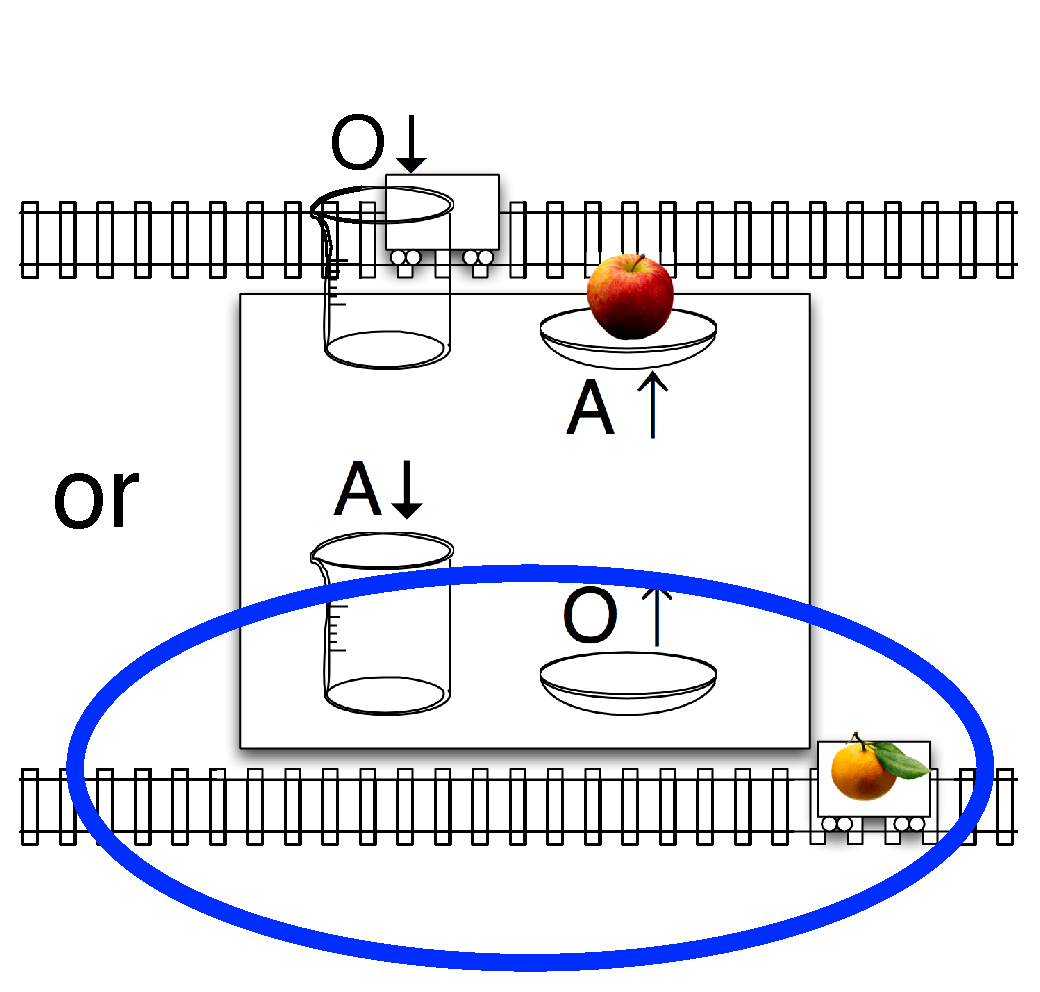
\includegraphics[height=0.8\textheight]{f5.eps}}
  \only<6>{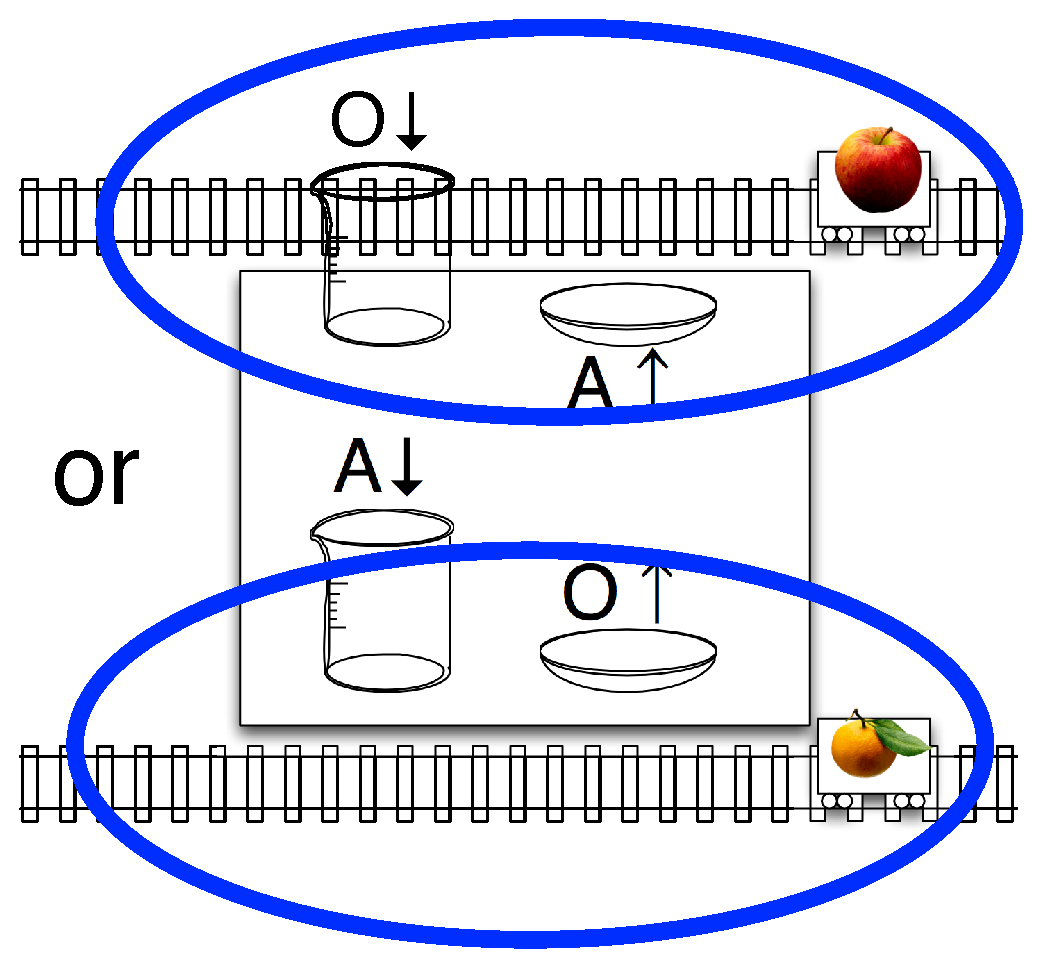
\includegraphics[height=0.8\textheight]{f6.eps}}
 \end{frame}

 \begin{frame}
  \frametitle{ダメット公理$(O\rightarrow  A)\lor (A\rightarrow O)$
  の実装に\\待ち合わせは不要}

  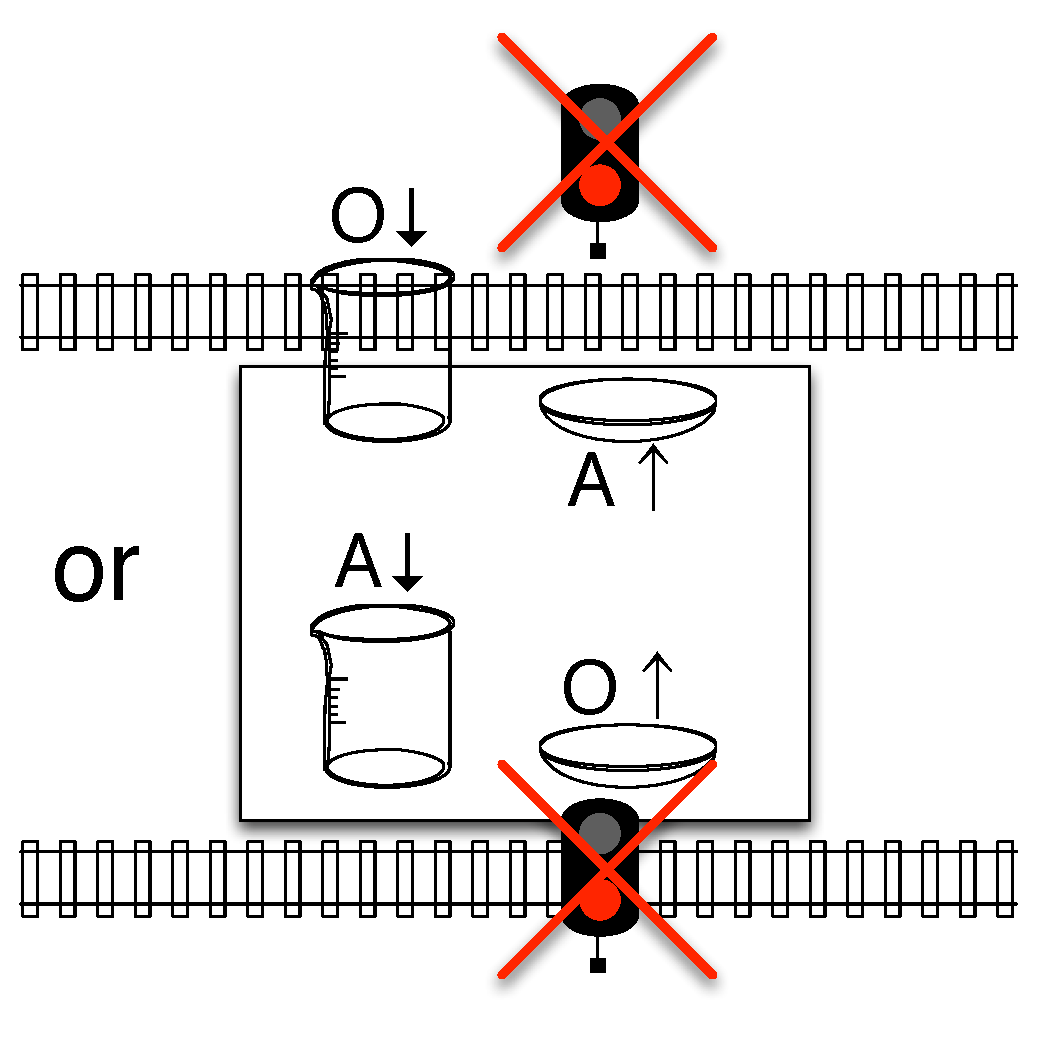
\includegraphics[height=0.8\textheight]{d.eps}
 \end{frame}

  \begin{frame}
   \frametitle{Implementation}
  \end{frame}

  \begin{frame}
   \frametitle{Results}
  \end{frame}

  \section{Parametricity}

  \begin{frame}
   \frametitle{Danos and Krivine}

   Similar interests.

   Possibly multiple components in executables.

   No communication among them.  Only\\
   (dist)
  \end{frame}

  \begin{frame}
   \frametitle{A Second Order Formulation}
   \aseq{\xphi,\G}{\tj t\psi}
   \LL{$\limp$I}
   \useq{\G}{\tj{\lambda x.t}{\phi\limp\psi}}
   \DisplayProof
   \hfill
   %
   \aseq{\G}{\tj t{\phi\limp\psi}}
   \aseq{\D}{\tj u\phi}
   \LL   {$\limp$E}
   \bseq{\G,\D}{\tj{(t)u}\psi}
   \DisplayProof
   \ruleskip
   %
   \aseq{\G}{\tj{t}{\phi}}
   \LL  {$\oplus$I}
   \useq{\G}{\tj{\inl{t}}{\phi\oplus\psi}}
   \DisplayProof
   \ruleskip
   %
   \aseq{\G}{\tj{t}{\phi\oplus\psi}}
   \aseq{\D,\xphi}{\tj{u_0}{\theta}}
   \aseq{\D,\ypsi}{\tj{u_1}{\theta}}
   \LL  {$\oplus$E}
   \tseq{\G,\D}{\tj{\mat{t}{x}{u_0}{y}{u_1}}{\theta}}
   \DisplayProof
   \ruleskip
   %
   \aseq\G{\tj t\phi}
   \LL   {$\forall$I}
   \useq\G{\tj t{\forall X\phi}}
   \DisplayProof (no free $X$ in $\G$)
   \hfill
   %
   \aseq{\G}{\tj{t}{\forall X\phi}}
   \LL   {$\forall$E}
   \useq{\G}{\tj{t}{\phi[\psi/X]}}
   \DisplayProof
   \ruleskip
   %
   \aseq{\tj{x}{\phi\limp\psi},\G}{\tj t\theta}
   \aseq{\tj{y}{\psi\limp\phi},\D}{\tj u\theta}
   \LL{Com}
   \bseq{\G,\D}{\tj{(t[\comodL/x]\conc u[\comodR/y])}{\theta}}
   \DisplayProof
   \ruleskip

   Note that Com rule introduces weakening on the left.\\
   \AxiomC{}
   \useq{\phi\limp\phi}{\phi\limp\phi}
   \aseq{\G}{\phi}
   \bseq{\phi\limp\phi,\G}{\phi}
   \AxiomC{}
   \useq{\phi\limp\phi}{\phi\limp\phi}
   \aseq{\G}{\phi}
   \bseq{\phi\limp\phi,\G}{\phi}
   \bseq{\G,\G}{\phi}
   \DisplayProof

   Note the com rule introduces left weakening.
  \end{frame}

  \begin{frame}
   \frametitle{An Easier Operational Semantics without Stores}
   \begin{description}
    \item[(cong)] if
	 $e_0         \red e_1$
	 then
	 $(e_0 \conc e) \red (e_1\conc e)$
    \item[(push)]
	 $[(t)u,\pi]      \red [t,u\cdot\pi]$
    \item[(store)]
	 $[\lambda x.t,u\cdot\pi]
	 \red
	 [t[\ast_u/x],      \pi]$
    \item[(load)]
	 $[\ast_u,\pi]\red [u,\pi]$
    \item[(dist)]
	 $[(t\conc u),\pi]  \red [t,\pi\conc u,\pi]$
    \item[(ask)]
	 $[\mat t x u y v,\pi]\red [t,\mats x u \pi y v \pi]$
    \item[(ansL)]
	 $[\inl{v}, \mats xt\pi yu\sigma] \red [t[v/x],\pi] $
    \item[(ansR)]
	 $[\inr{w}, \mats xt\pi yu\sigma] \red [u[w/y],\sigma] $
    \item[(com0)]
	 $[\comod c{\co c}, t\cdot\pi\conc \comod{\co c}c,
	 u\cdot\sigma] \red
	 [u,\pi]$\enspace(if $\co c\sche c$ but $c\not\sche \co c$)
    \item[(com1)]
	 $[\comod c{\co c}, t\cdot\pi\conc \comod{\co c}c,
	 u\cdot\sigma] \red
	 [t,\sigma]$\enspace(if $c\sche \co c$ but $\co c\not\sche c$)
    \item[(com2)]
	 $[\comod c{\co c}, t\cdot\pi\conc \comod{\co c}c,
	 u\cdot\sigma] \red
	 [u,\pi\conc t,\sigma]$\enspace(if $c\sche \co c$ and $\co c\sche
	 c$)\enspace.
   \end{description}
  \end{frame}

  \begin{frame}
   \frametitle{Goal: Specification Problem}
   \begin{proposition}
    \label{prop:spec}
    Let
    $\sequent{}{}{\tj c
    {\forall X\forall A\forall B
    [((A\limp B)\limp X)
    \limp((B\limp A)\limp X)
    \limp X]}}$
    be
    derivable;
    $\rho,\sigma, r$ terms and $\pi, \pi_A,
    \pi_B$ stacks. \\
    Given $[(\rho)d  ,\pi]\red [d,a\cdot \pi_B]$ and
    $[(\sigma)f,\pi]\red [f,b\cdot \pi_A]$ for all $d, f$,\\
    $[(c)(\rho)\sigma,\pi]$ reduces to a multiset containing an
    element of
    $\{(a,\pi_A),(b,\pi_B)\}$.
   \end{proposition}
  \end{frame}

  \begin{frame}
   \frametitle{Assigining Meaning to Types}
   For a set~$\mathcal Z$ of stacks, $\mathcal Z\rightarrow\bbot$ denotes
   the set of terms~$t$ such that
   for any stack $\pi\in \mathcal Z$,
   the executable $t,\pi$ is in $\bbot$.

   For $\phi\in\form(2^\Pi)$ and $|\cdot|^-_0\colon\pvar\rightarrow 2^\Pi$,
   we define $\nsem{\phi}\colon
   2^\Pi$ as
   \begin{align*}
    \nsem{\mathcal Z} &= \mathcal Z \\
    \nsem{X}&= |X|_0^- \\
    \nsem{\phi\limp\psi}&=
    \{t\cdot\pi\mid
    t\in\nsem\phi\rightarrow\bbot \text{ and }\pi\in\nsem\psi\}\\
    \nsem{\phi\oplus\psi}=& \{\mats x{t}{\pi}y{u}{\sigma}\mid\\ &
    t[v/x],\pi\in\bbot \text{ for all } v\in\nsem{\phi}\rightarrow\bbot\text{
    and }\\ &
    u[w/y],\sigma\in\bbot \text{ for all } w\in\nsem{\psi}\rightarrow\bbot\}
    \\
    \nsem{\forall X\phi}=&
    \bigcup_{\mathcal Z\in 2^\Pi} \nsem{\phi[\mathcal Z/X]}\enspace.
   \end{align*}
   Using this, we define $\sem \phi=\nsem{\phi}\rightarrow\bbot$.
  \end{frame}

  \begin{frame}
   \frametitle{Goal: Adequacy}

   \begin{proposition}[?]
    Let
    $  \sequent{\G}{\tj{t}{\phi}} $ be derivable.\\
    The term
    $
    t[\vec{g}/\G]
    $
    is in $\sem\phi$
    for any
    $\vec{g}\in\sem{\G}$.
   \end{proposition}

   \structure{Proof attempt.}
   By induction on \#steps of derivations.

   Com gets stuck.
   \fix{how}
  \end{frame}

  \begin{frame}
   \frametitle{Adequacy on Two Derivations}
   \begin{proposition}[Adequacy]
    Let these sequents be derivable:
    $  \sequent{\G}{\tj{t}{\phi}} $
    and
    $  \sequent{\D}{\tj{u}{\psi}}$\enspace.
    \\Under these conditions, we state that:
    \begin{enumerate}
     \item the term
	   $
	   t[\vec{g}/\G]
	   $
	   is in $\sem\phi$
	   for any
	   $\vec{g}\in\sem{\G}$; and that
     \item \label{prop}
	   when $\G$ and $\D$ are respectively
	   equal to $\tj x\theta, \hat\G$ and $\tj y\tau, \hat\D$ up to exchange,
	   the following pair is in $\sempair{\phi,\psi}$:
	   \[\left(
	   t[v/x][\vec g/\hat \G],\quad
	   u[w/y][\vec d/\hat \D]
	   \right)
	   \]
	   for any
	   $(v,w)\in\sempair{\theta,\tau}$,
	   $\vec g\in\sem{\hat\G}$ and
	   $\vec d\in\sem{\hat\D}$.
    \end{enumerate}
    where $(v,w)\in \sempair{\phi,\psi}\Longleftrightarrow v,\pi_\phi\conc
    w,\pi_\psi \in \bbot$
   \end{proposition}
   By induction on the sum of \#steps of
   derivations, \ldots\\
   the $\limp$E case gets stuck for \ref{prop}.
  \end{frame}

  \begin{frame}
   \frametitle{Adequacy: the Final Form}
   \begin{proposition}[Adequacy]
    Let these sequents be derivable:
    $  \sequent{\G}{\tj{t}{\phi}} $
    and
    $  \sequent{\D}{\tj{u}{\psi}}$\enspace.
    \\Under these conditions, we state that:
    \begin{enumerate}
     \item the program
	   $
	   (t[\vec{g}/\G], \alert{e})
	   $
	   is in $\sem\phi$
	   for any
	   $(\vec{g},\alert{e})\in\sem{\G}$; and that
     \item
	  when $\G$ and $\D$ are respectively
	  equal to $\tj x\theta, \hat\G$ and $\tj y\tau, \hat\D$ up to exchange,
	  the following \alert{triple} is in $\sempair{\phi,\psi}$:
	  \[\left(
	  t[v/x][\vec g/\hat \G],\quad
	  u[w/y][\vec d/\hat \D],\quad
	  \alert{e \conc  f \conc e'}
	  \right)
	  \]
	  for any
	  $(v,w,\alert{e'})\in\sempair{\theta,\tau}$,
	  $(\vec g, \alert{e})\in\sem{\hat\G}$ and
	  $(\vec d, \alert{f})\in\sem{\hat\D}$.
    \end{enumerate}
   \end{proposition}
   where
  \end{frame}

  \begin{frame}
   An \textit{environment} $(t,\pi)\in E = \Lambda\times\Pi$\\
   For a set~$\mathcal Z$ of environments, $\mathcal Z\rightarrow\bbot$ denotes
   the set of programs $(t,e)$ such that
   for any environment $(\pi,e')\in \mathcal Z$,
   the executable $t,\pi\conc e \conc e'$ is in $\bbot$.

   For $\phi\in\form(2^E)$ and $|\cdot|^-_0\colon\pvar\rightarrow 2^E$,
   we define $\nsem{\phi}\colon
   2^E$ as
   \begin{align*}
    \nsem{\mathcal Z} &= \mathcal Z \\
    \nsem{X}&= |X|_0^- \\
    \nsem{\phi\limp\psi}&=
    \{(t\cdot\pi, e_0\conc e_1)\mid
    (t,e_0)\in\nsem\phi\rightarrow\bbot \text{ and }(\pi,e_1)\in\nsem\psi\}\\
    \nsem{\phi\oplus\psi}=& \{(\mats x{t}{\pi}y{u}{\sigma}, f)\mid\\ &
    t[v/x],\pi\conc f\conc f'\in\bbot \text{ for all } (v,f')\in\nsem{\phi}\rightarrow\bbot\text{
    and }\\ &
    u[w/y],\sigma\conc f\conc f'\in\bbot \text{ for all } (w,f')\in\nsem{\psi}\rightarrow\bbot\}
    \\
    \nsem{\forall X\phi}=&
    \bigcup_{\mathcal Z\in 2^\Pi} \nsem{\phi[\mathcal Z/X]}\enspace.
   \end{align*}
   Using this, we define $\sem \phi=\nsem{\phi}\rightarrow\bbot$.
  \end{frame}

  \begin{frame}
   \frametitle{Todo}
   \begin{itemize}
    \item Add exponentials or intuitionistic implication.
    \item Try the technique of communication encapsulation $\sempair{\phi,\psi}$ on process calculi.
   \end{itemize}
  \end{frame}

\end{document}